\chapter{Mediciones}

\section{Introducción}

En este capítulo se detallarán las mediciones realizadas sobre el prototipo. Se
explicará el banco de mediciones conformado, con todos sus componentes. Se
discutirá el desempeño medido del sistema en el contexto de los resultados
reportados en la literatura. Al final del capitulo, se presentan una tabla y un
gráfico comparando el desempeño obtenido con el reportado en otros trabajos.

\section{Banco de medición}

En la Figura \ref{fig:banco_medicion} puede observarse un diagrama del banco de
medición. Consiste de los siguientes bloques:

\begin{itemize}
    \item Placa FPGA: genera un pulso cuadrado unipolar, de frecuencia y ciclo
      de trabajo configurables. Con la frecuencia se controla la $PRF$ de los
      pulsos de salida, y con el ciclo de trabajo los valores de tensión del
      pulso de salida del \textit{driver}.
    \item Fuente de alimentación: provee la alimentación $V_{dd}$ para el
     \textit{driver}. El valor de esta tensión determina la amplitud pico a pico del
      pulso de salida del \textit{driver}.
    \item \textit{Driver}: cumple la función de \textit{buffer} para la
	FPGA, presentando una alta impedancia a la salida de la misma.
      Convierte el pulso unipolar de \qty{3.3}{\volt} en uno bipolar, con
      amplitud pico a pico igual a $V_{dd}$ (\qty{5}{\volt} o \qty{7}{\volt}).
    \item \textit{Pulser}: el DUT, genera pulsos ultra cortos en base 
      a la salida del driver.
    \item Osciloscopio: instrumento de medición del experimento. Actúa como
      carga con su impedancia de entrada de \qty{50}{\ohm}.
\end{itemize}

\begin{figure}[t!]
  \centering
    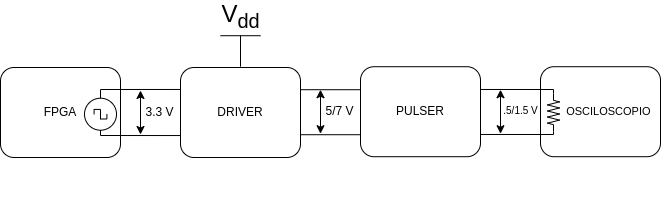
\includegraphics[width=1\textwidth]{images/banco_medicion.drawio.png}
    \caption{Banco de medición}
    \label{fig:banco_medicion}
\end{figure}

\subsection{Fuente de alimentación}

Para la fuente de alimentación se utilizó una \textit{Marconi Instruments
TF2154}, en la figura \ref{fig:mediciones_fuente} puede observarse la misma.

Presentaba limitación de corriente regulable e indicadores para la amplitud y la
corriente suministrada, lo que permitía trabajar de manera segura, dentro de los
límites de consumo obtenidos en las simulaciones anteriores.

Como fuese explicado en la sección \ref{sec:pulser_power}, la corriente máxima
esperada en las condiciones de trabajo era menor a \qty{200}{\milli\ampere}, por
lo que se monitoreó durante todo el experimento que la corriente entregada por
la fuente no supere este máximo teórico.

\begin{figure}[t!]
    \begin{minipage}[t]{0.5\linewidth}
      \centering
        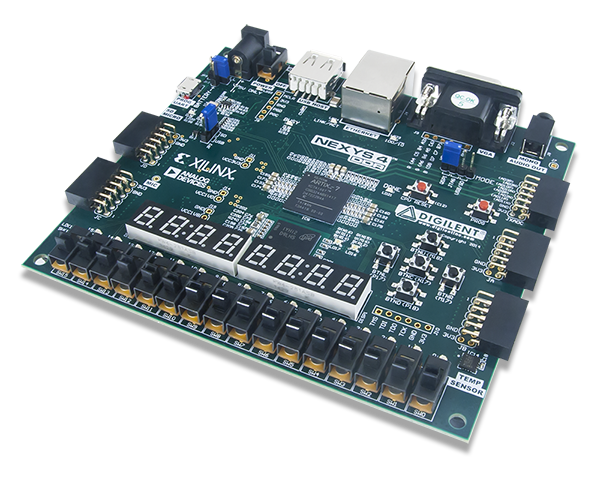
\includegraphics[width=1\textwidth]{images/mediciones_fpga.png}
        \caption{Placa de desarrollo FPGA para generación de señal de control.}
        \label{fig:mediciones_fpga}
    \end{minipage}
    \hfill
    \begin{minipage}[t]{0.5\linewidth}
        \centering
        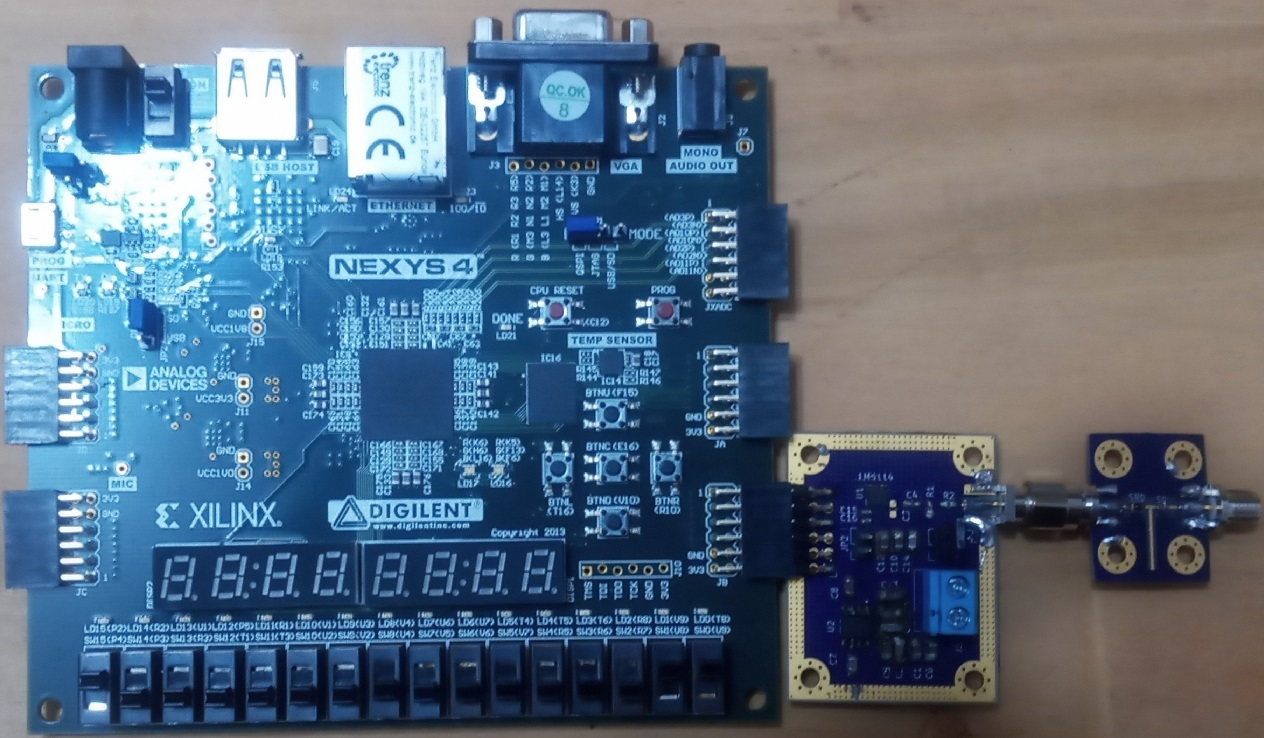
\includegraphics[width=1\textwidth]{images/sistema_medido_small.jpg}
        \caption{FPGA, \textit{driver} y \textit{pulser}.}
        \label{fig:sistema_medido}
    \end{minipage}
\end{figure}

\subsection{FPGA}

La FPGA generaba el pulso unipolar cuadrado de entrada, que controlaba la
$PRF$ y el ciclo de trabajo del pulso del driver. La placa utilizada fue
\textit{Nexys-4 DDR} de Digilent \cite{digilent_nexys4ddr}, con un chip
\textit{Artix-7} de Xilinx. En la figura \ref{fig:mediciones_fpga} puede
observarse la misma. 

Se utilizó una FPGA para poder validar la utilidad del prototipo en el contexto
de un sistema UWB como el descripto en \cite{altieri2017}, en el que se dispone
de señales de control digitales. Este componente del sistema es fácilmente
reemplazable por otra FPGA o sistema embebido. Las variables de ajuste del pulso
unipolar de la FPGA eran las siguientes

\begin{itemize}
  \item Frecuencia: la frecuencia de la señal cuadrada de entrada es igual a la
    frecuencia de repetición de pulsos ($PRF$) del sistema, ya que controla la
    frecuencia con la que el SRD se prende y se apaga y, por lo tanto,
    la frecuencia de generación de pulsos.
  \item Ciclo de trabajo: el ciclo de trabajo de la señal cuadrada unipolar
    determina los extremos de tensión de la señal cuadrada bipolar de salida del
    driver. A mayor ciclo de trabajo, valores más negativos. Este control se da
    a través del control del valor medio de la señal, que luego es restado por
    el capacitor serie del \textit{driver}.
\end{itemize}

\textbf{Diseño implementado:}

El diseño implementado en la FPGA consistía en un generador de cuadrada con
ciclo de trabajo y frecuencia variables. La interfaz del sistema era la
siguiente

\begin{itemize}
  \item Los botones \textit{BTNL} y \textit{BTNR} controlaban el ciclo de
    trabajo en pasos de a \qty{1}{\percent} en incrementos y decrementos
    respectivamente.
  \item Los botones \textit{BTND} y \textit{BTNU} controlaban el ciclo de
    trabajo en pasos de a \qty{10}{\percent} en incrementos y decrementos
    respectivamente.
  \item Con los \textit{switches} \textit{SW0} a \textit{SW1} se controlaba la
    frecuencia del pulso unipolar.
    \begin{itemize}
      \item Con \textit{SW0} seleccionado, la frecuencia era de
        \qty{1}{\mega\hertz}.
      \item Con \textit{SW1} seleccionado, la frecuencia era de
        \qty{5}{\mega\hertz}.
      \item Con \textit{SW2} seleccionado, la frecuencia era de
        \qty{10}{\mega\hertz}.
    \end{itemize}
\end{itemize}

En el anexo \ref{app:verilog} se encuentra el HDL del diseño implementado.

\subsection{Osciloscopio}

El osciloscopio fue utilizado para realizar la medición en el dominio del tiempo
del pulso generado. Para una medición exitosa, era indispensable que este
instrumento cuente con los requerimientos de ancho de banda del pulso. Como
fuese explicado en \ref{sec:pulse_bandwidth}, el ancho de banda esperado para el
pulso era de \qty{3.5}{\giga\hertz}.

El osciloscopio utilizado fue un \textit{Tektronix MSO 70404C}, en la figura 
\ref{fig:osciloscopio} puede observarse el mismo. El instrumento posee 
\qty{4}{\giga\hertz} de ancho de banda analógico, y una tasa de muestreo
de \qty[per-mode=symbol]{25}{\giga\siemens\per\second}, con la posibilidad de
realizar muestreo en tiempo equivalente \cite{oscilloscope_datasheet}. Estas
prestaciones eran suficientes para medir el pulso de salida.

El instrumento posee configuraciones de impedancia de entrada seleccionables entre
\qty{50}{\ohm} y \qty{500}{\mega\ohm} \cite{oscilloscope_datasheet}. Para la
medición del prototipo, se seleccionó la entrada de \qty{50}{\ohm}, actuando
esta impedancia como carga del generador de pulsos.

\begin{figure}[t!]
    \centering
    \begin{minipage}{0.45\linewidth}
        \centering
        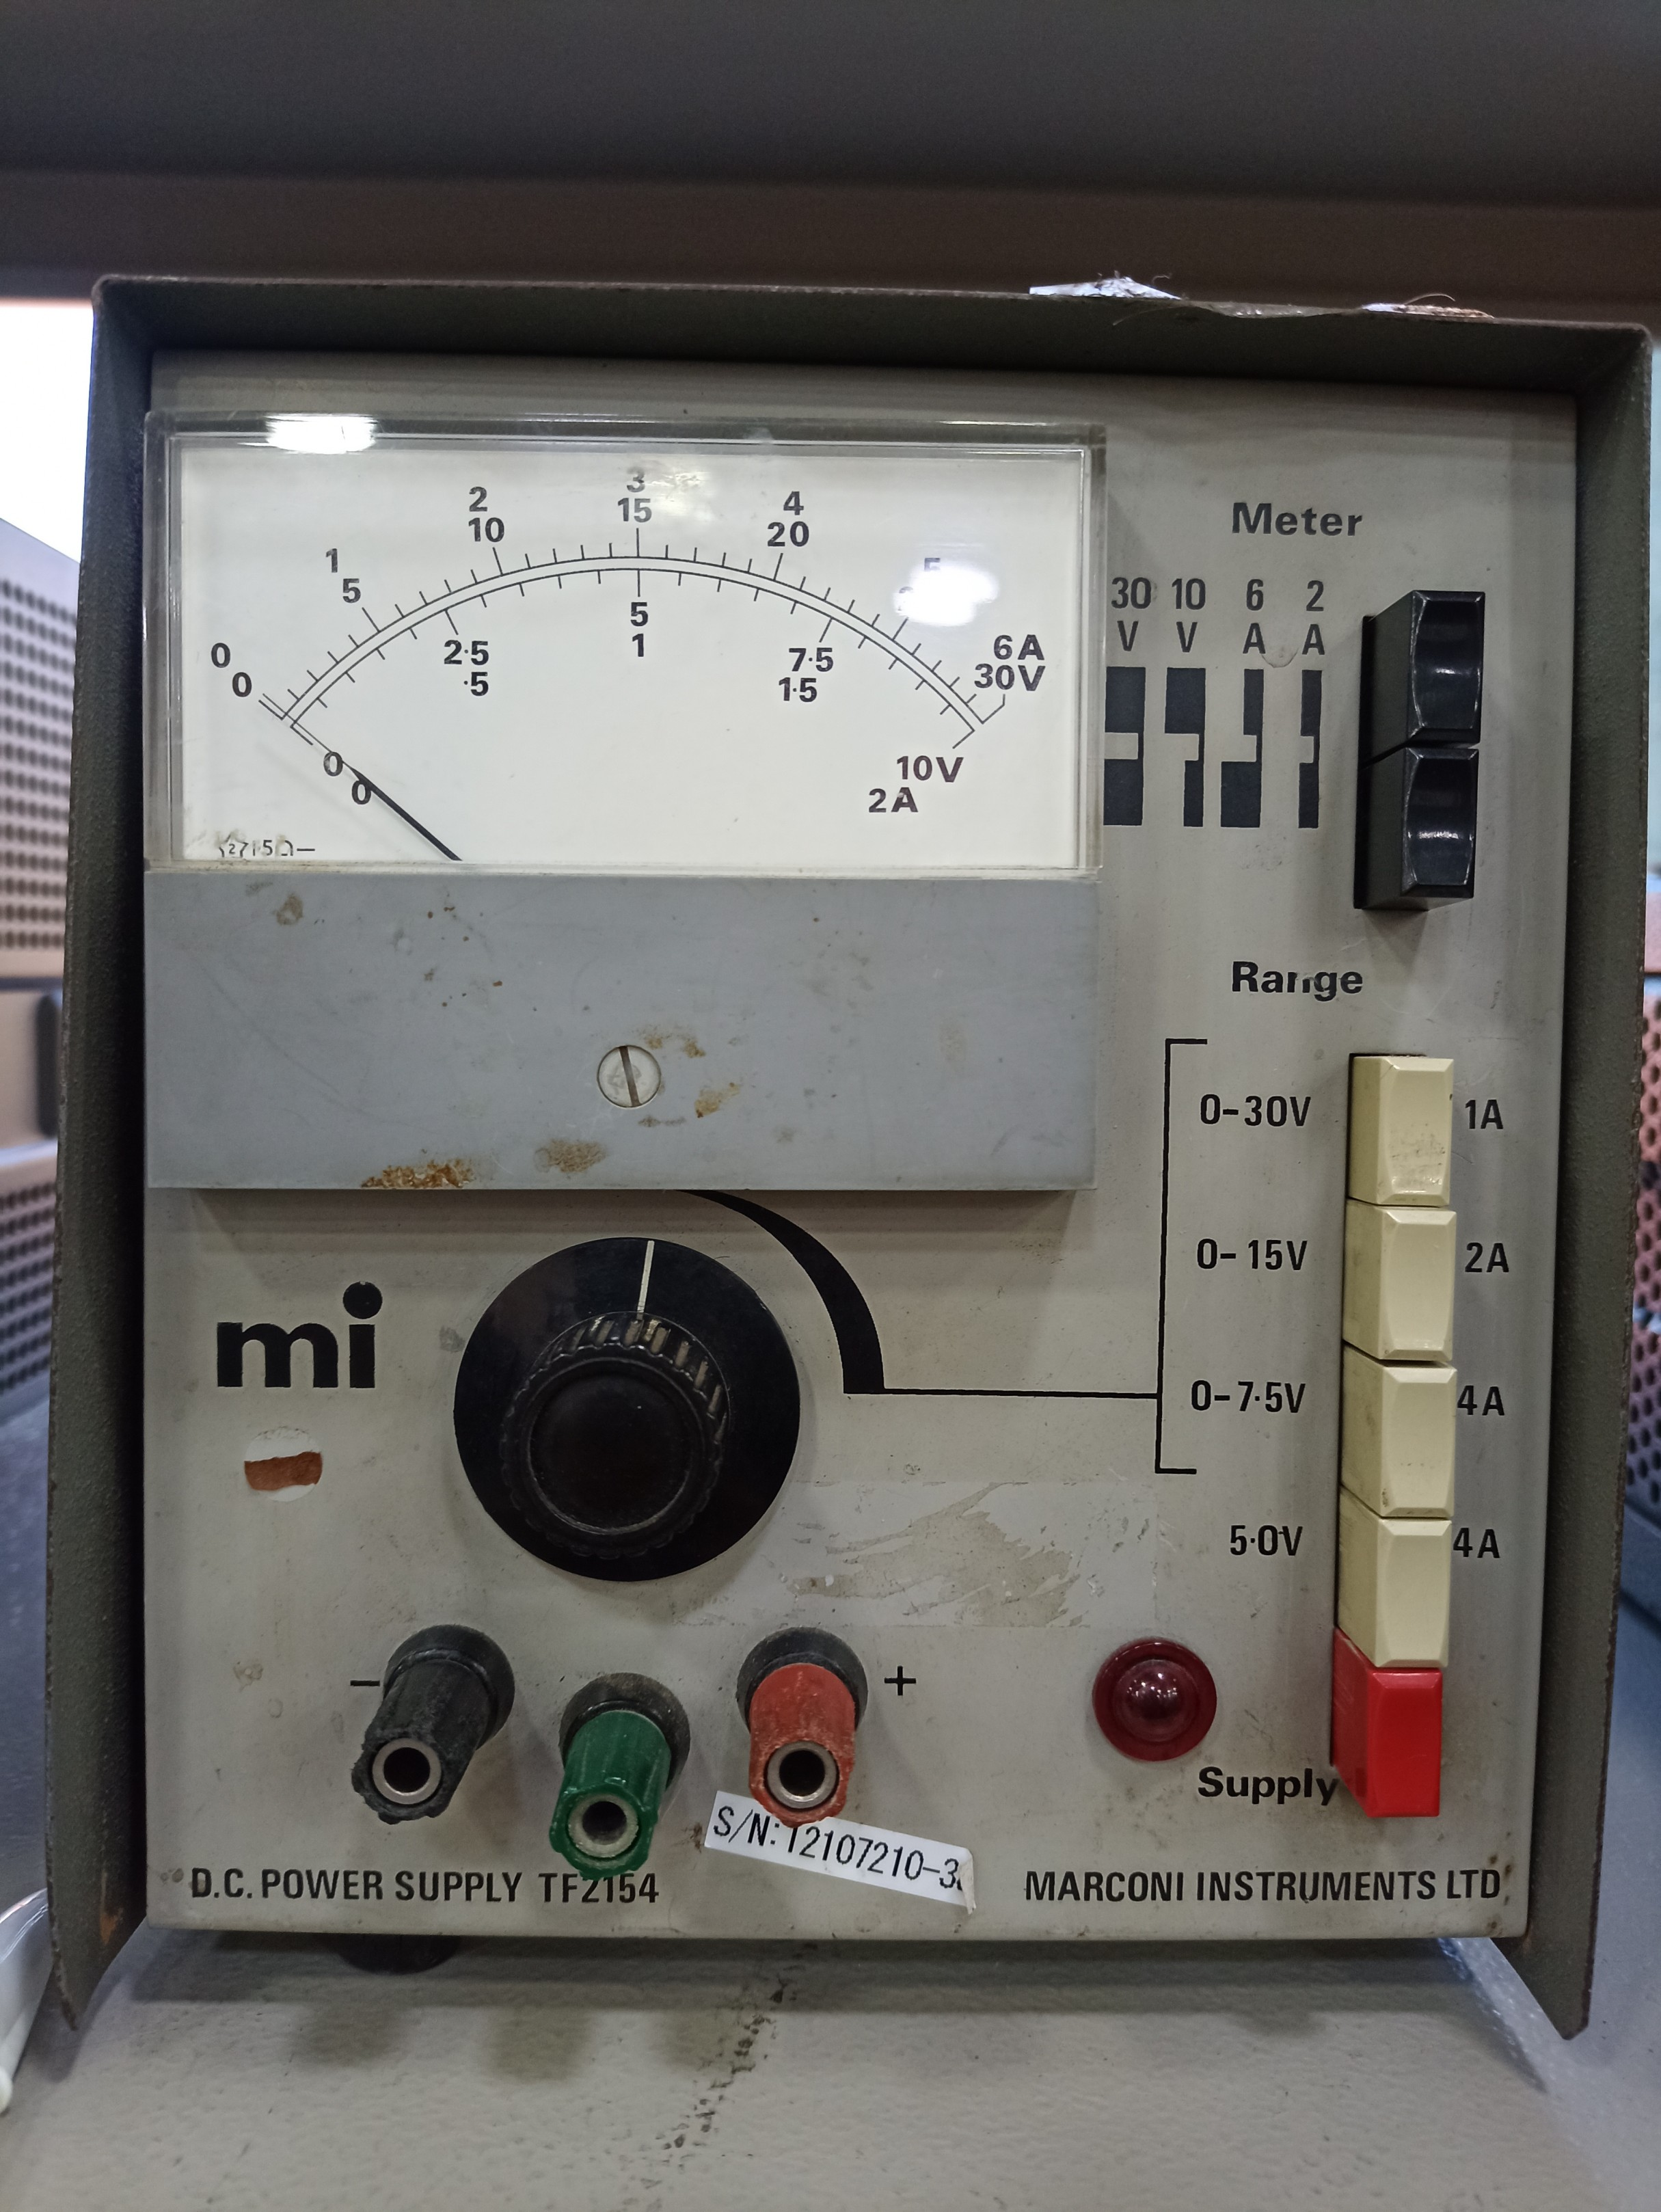
\includegraphics[trim=0 10cm 0 20cm, clip, width=.8\textwidth]{images/mediciones_fuente.jpg}
        \caption{Fuente utilizada para alimentar el prototipo.}
        \label{fig:mediciones_fuente}
    \end{minipage}
    \hfill
    \begin{minipage}{0.45\linewidth}
        \centering
        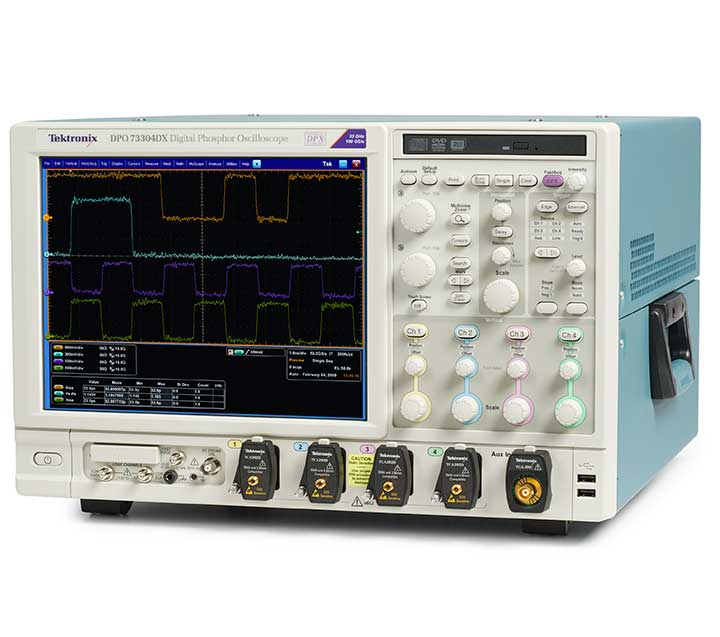
\includegraphics[width=0.95\textwidth]{images/osciloscopio.png}
        \caption{Osciloscopio \textit{Tektronix MSO 70404C} utilizado para la medición del pulso.}
        \label{fig:osciloscopio}
    \end{minipage}
\end{figure}

\subsection{Seguridad del instrumento}

Debido a las prestaciones del osciloscopio y su gran costo, era fundamental
garantizar la integridad del mismo en la medición del experimento. Dado que
actuaba como carga del DUT, se debía garantizar que bajo todas las condiciones
de trabajo, la potencia entregada por el generador de pulsos se encuentre dentro
de los límites determinados por el fabricante del equipo para evitar posibles
daños.

La máxima tensión de entrada se especifica en $5\text{V}_{RMS}$ para una
resolución $\geq100m\text{V}/\text{div}$ y $1 \text{V}{RMS}$ para una resolución
$<100 m\text{V}/\text{div}$.  Para garantizar la seguridad del equipo en
cualquier caso, se toma como límite el valor de peor caso, $1\text{V}_{RMS}$
(correspondiente a una resolución $\geq 100 m\text{V/div}$, para resoluciones
menores a esta el límite es mayor).

En condiciones normales de funcionamiento, la potencia disipada por la carga es
mínima, ya que es la potencia que disipa el tren de pulsos en un carga de
\qty{50}{\ohm}. Como fuese desarrollado en la sección \ref{sec:pulser_power},
esta potencia está acotada por \qty{0.3}{\milli\watt}, que en \qty{50}{\ohm}
resultan en \qty{123}{\milli\voltRMS}, que se encuentran muy por debajo de los
\qty{1}{\voltRMS} especificados por el fabricante.

No solo es necesario analizar la disipación de potencia en condiciones normales
de funcionamiento, sino también para el caso de una falla, ya que el principal
objetivo es garantizar la integridad del instrumento en cualquier condición.

En caso de ocurrir alguna falla con algún componente del circuito, el \textit{stub}
de salida provee una función de protección. Este componente, para señales con
una variación temporal mucho mayor al largo del mismo, actúa como una puesta a
tierra.

Entonces, la componente de continua a la salida del generador de pulsos tiene un
valor esperado de \qty{0}{\volt}, tanto para condiciones normales de 
funcionamiento como en presencia de fallas.

En cuanto a la componente alterna de la salida, su valor esperado es
extremadamente bajo, ya que únicamente señales de gran ancho de banda pueden ser
filtradas y permanecer con una amplitud considerable a la salida del 
\textit{stub}.

\section{Mediciones realizadas}

Las mediciones consistieron en mediciones en el dominio del tiempo del pulso de
salida. Utilizando funciones provistas por el osciloscopio, se midieron tiempo
de crecimiento, tiempo de decaimiento, amplitud máxima, y ancho a medio máximo
(FWHM del inglés \textit{Full Width at Half Maximum}).

Se realizaron distintas mediciones para distintas condiciones de trabajo del
circuito. Se barrió para el pulso digital de entrada, el ciclo de trabajo, y
para la fuente de alimentación distintos valores de tensión.

\begin{itemize}
    \item Para la amplitud de la fuente, se utilizaron valores de \qty{5}{\volt} y
        \qty{7}{\volt}.
        \begin{itemize}
            \item \qty{5}{\volt} por ser un valor fácilmente obtenible en los
                sistemas {UWB} de referencia.
            \item \qty{7}{\volt} por ser la máxima amplitud tolerable por el circuito.
                Tensiones de alimentación mayores a estas resultan en corrientes de
                polarización mayores a las máximas admisibles dado los
                dimensionamientos de las pistas de los {PCBs}.
        \end{itemize}
    \item El ciclo de trabajo se barrió entre \qty{50}{\percent} y
        \qty{70}{\percent}.
        \begin{itemize}
            \item Se tomo 50\% como límite inferior por ser un valor fácilmente
                obtenible como división de un reloj digital.
            \item Se tomo 70\% como límite superior ya que se observó que valores
                superiores a este resultaban en un pulso bipolar con amplitudes
                negativas decrecientes, y por lo tanto, amplitudes de pulso
                decrecientes.
            \item La teoría no indicaba un límite superior para el ciclo de
                trabajo. Sin embargo, este se observó en la práctica debido al
                comportamiento no ideal del pulso de salida del \emph{driver},
                que no era perfectamente cuadrado.
        \end{itemize}
\end{itemize}

En la figura \ref{fig:sistema_medido} puede observarse el \textit{pulser} junto con el
\textit{driver} y la FPGA.

\subsection{Mediciones del \textit{driver}}

\begin{figure}[t!]
    \begin{minipage}[t]{0.45\linewidth}
        \centering
        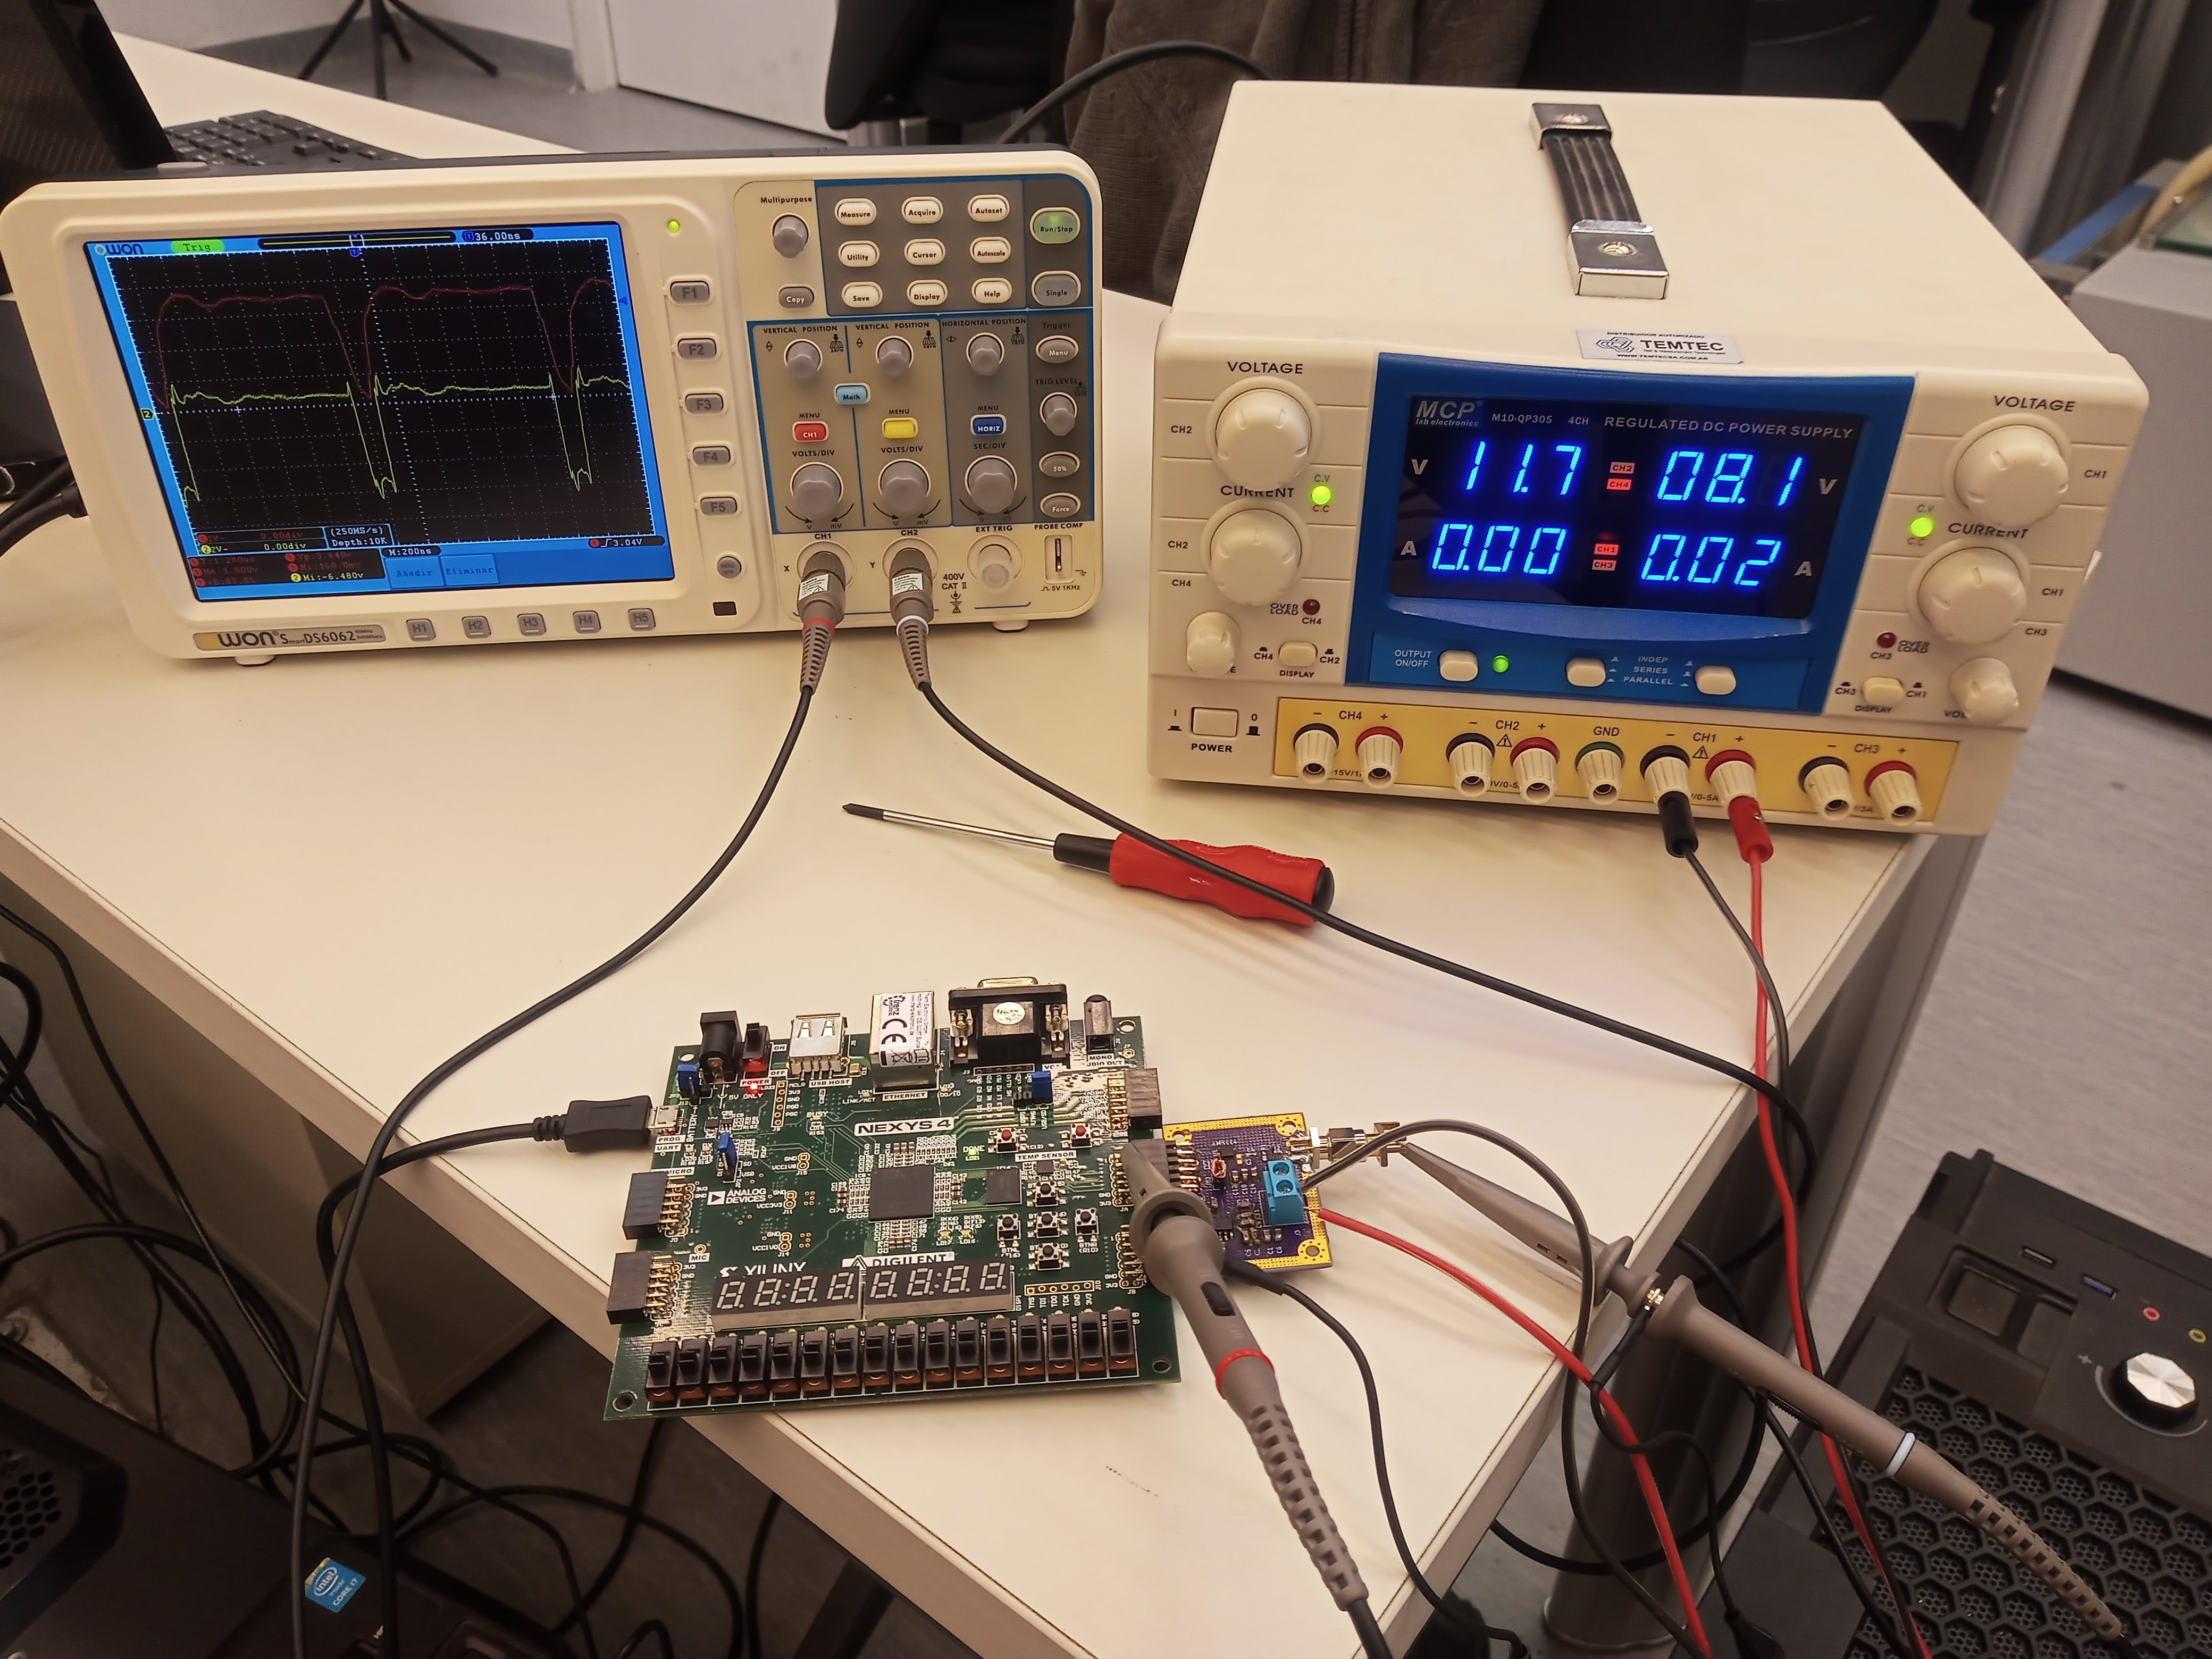
\includegraphics[trim=0 1cm 0 0.5cm, clip, width=1\textwidth]{images/banco_pre_mediciones.jpg}
        \caption{Banco de medición para el \textit{driver}.}
        \label{fig:banco_pre_mediciones}
    \end{minipage}
    \hfill
    \begin{minipage}[t]{0.45\linewidth}
        \centering
        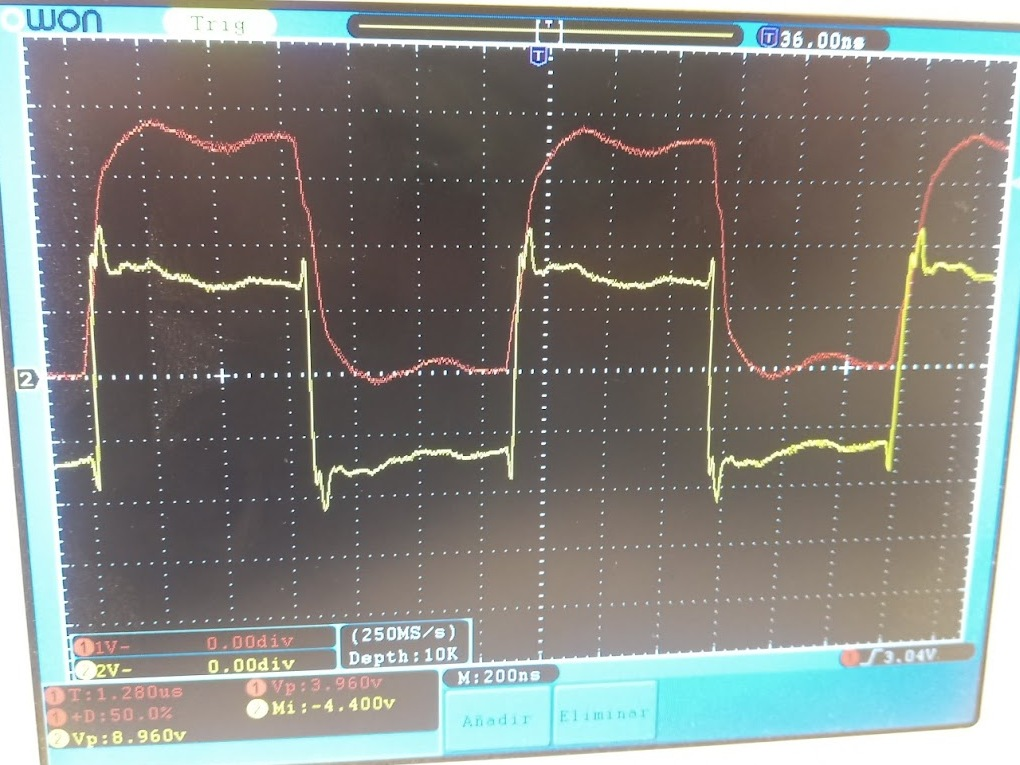
\includegraphics[width=1\textwidth]{images/medicion_driver_D_50.jpg}
        \caption{Medición de driver para $D= \qty{50}{\percent}$}
        \label{fig:medicion_driver_D_50}
    \end{minipage}
\end{figure}

Previo a las mediciones principales, se realizó una medición de la salida del driver,
con el objetivo de validar el pulso bipolar generado.

El motivo de esta medición previa fue la limitada disponibilidad del
osciloscopio de gran ancho de banda utilizado para la medición final del pulso.
Esta pre-medición del pulso bipolar se realizó con un osciloscopio de bajo ancho
de banda, ya que el objetivo era validar los niveles de tensión del pulso, y su
correcta variación con la variación del ciclo de trabajo del pulso unipolar.

En la figura \ref{fig:banco_pre_mediciones} puede observarse el banco de
medición. Se utilizó la FPGA para generar el pulso cuadrado unipolar, y se
conectó la punta de un osciloscopio a los terminales de un conector SMA
conectado a la salida del \textit{driver}. La entrada del osciloscopio se
configuró en alta impedancia. La alimentación la proveyó una fuente de continua
como se observa en la figura \ref{fig:banco_pre_mediciones}, con una
alimentación de \qty{8}{\volt}. El osciloscopio utilizado en este caso no fue el
Tektronix MSO 70404C de gran ancho de banda, sino uno comercial de
\qty{50}{\mega\hertz}.

En las figuras \ref{fig:medicion_driver_D_50}, \ref{fig:medicion_driver_D_71} y
\ref{fig:medicion_driver_D_92} se observan los resultados obtenidos para distintas
condiciones de ciclo de trabajo. En rojo se muestra la salida de la FPGA y en
amarillo la salida del driver. Abajo y a la izquierda de las formas de onda,
se observan la mediciones configuradas en el osciloscopio. La cantidad $V_p$ se
corresponde a la amplitud pico-a-pico, $+D$ al ciclo de trabajo y $M_i$ al valor
mínimo.

Para la salida de la FPGA se observa que la escala es de \qty{1}{\volt} por
división, notándose que la señal conmuta entre \qty{0}{\volt} y
\qty{3.3}{\volt}. El valor pico a pico es ligeramente mayor, alrededor de
\qty{3.8}{\volt} debido a sobrepicos presentes en la señal. El mismo comentario
aplica para la salida del driver, que está alimentado por \qty{8}{\volt}, pero
presenta una amplitud pico a pico de casi \qty{9}{\volt} debido a sobrepicos.

En la tabla \ref{tab:mediciones_driver_resultados} se resumen los resultados
obtenidos. Se observa una buena coincidencia entre los valores medidos y los
predecidos. Es de interés destacar que para la porción negativa del pulso, se
observa un sobrepico negativo, y que para mayores ciclos de trabajo, este
sobrepico representa casi la totalidad del período negativo.

En cuanto al valor positivo de la salida, es interesante notar que para el ciclo
de trabajo de \qty{92}{\percent}, notando que la escala es de \qty{2}{\volt}, se
observa un valor que oscila entre \qty{400}{\milli\volt} y
\qty{800}{\milli\volt}. Este valor no es suficiente para polarizar en directa al
SRD, por lo que quedan descartados ciclos de trabajo superiores a este valor
para operar el pulser.

\begin{figure}[t!]
    \begin{minipage}[t]{0.45\linewidth}
        \centering
        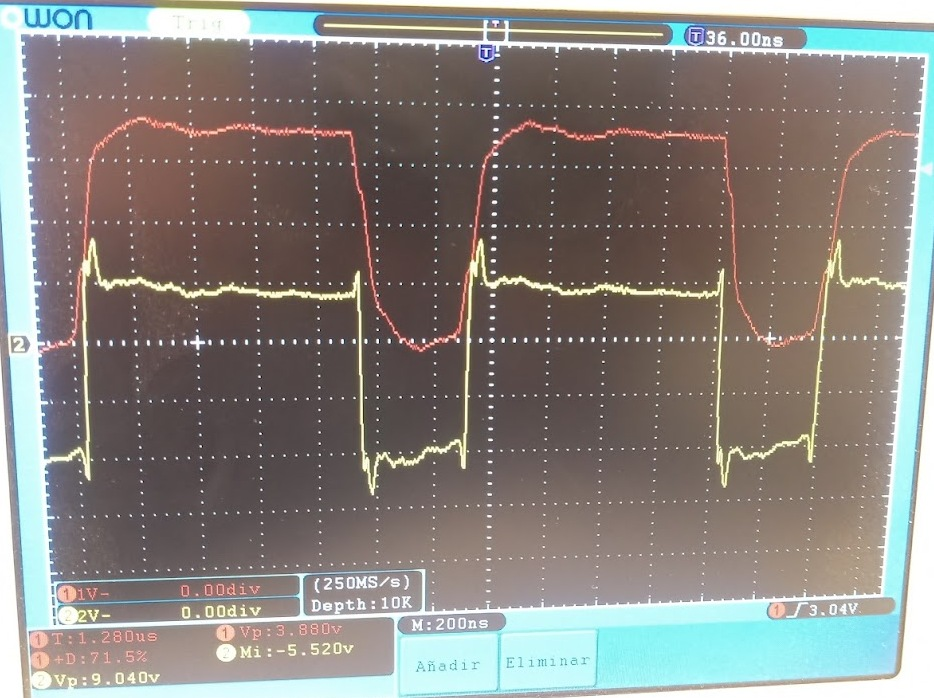
\includegraphics[width=1\textwidth]{images/medicion_driver_D_71.jpg}
        \caption{Medición de driver para $D= \qty{71}{\percent}$}
        \label{fig:medicion_driver_D_71}
    \end{minipage}
    \hfill
    \begin{minipage}[t]{0.45\linewidth}
        \centering
        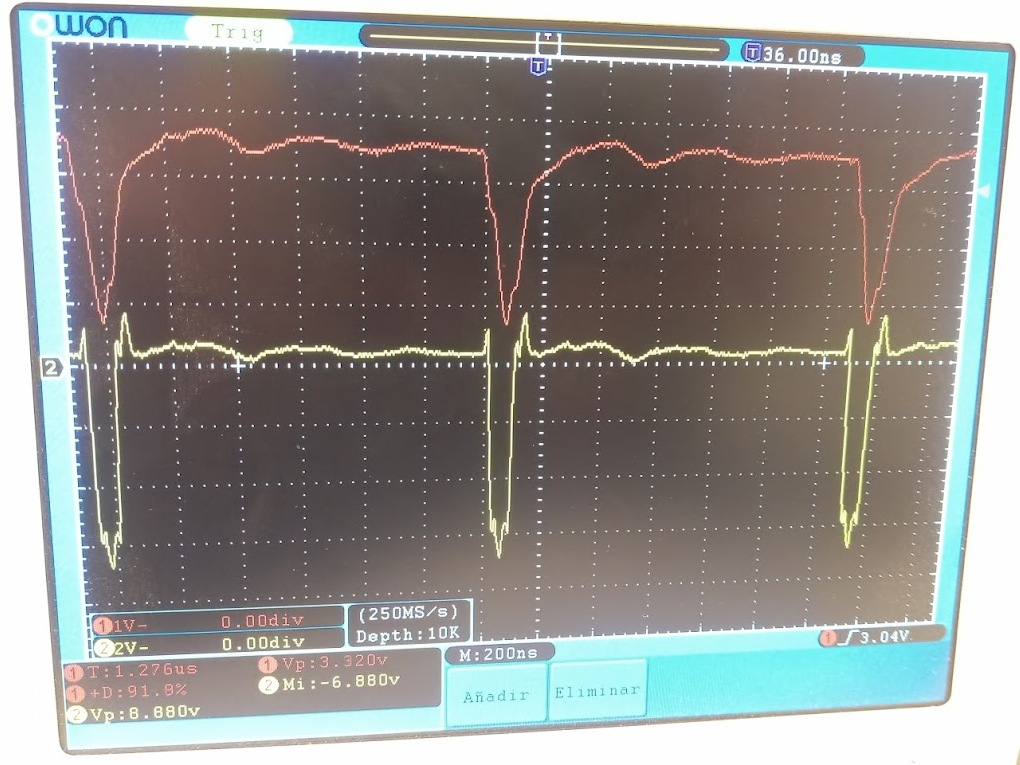
\includegraphics[width=1\textwidth]{images/medicion_driver_D_92.jpg}
        \caption{Medición de driver para $D= \qty{92}{\percent}$}
        \label{fig:medicion_driver_D_92}
    \end{minipage}
\end{figure}

\begin{table}[t!]
    \centering
    \begin{threeparttable}[b]
        \begin{tabular}{ccc}
        \hline
            $D$ [\unit{\percent}] & $V_{-m}$ \tnote{a} & $V_{-e}$ \tnote{b} \\
        \hline
            50 & 4.4 & 4.5 \\
            71 & 5.52 & 5.68 \\
            92 & 6.884 & 7.36  \\
        \hline
    \end{tabular}
    \begin{tablenotes}
        \item [a] $V_-$ medido
        \item [b] $V_-$ esperado según \ref{eq:v_minus_ideal_load}
    \end{tablenotes}
    \end{threeparttable}
    \caption{Resultados de medición de \textit{driver}}
    \label{tab:mediciones_driver_resultados}
\end{table}

\subsection{Medición de pulso}

En las figuras \ref{fig:mediciones_5v} y \ref{fig:mediciones_7v} se observan las
mediciones realizadas para $V_{cc}$ de \qty{5}{\volt} y \qty{7}{\volt}
respectivamente. En ambos casos, se realizaron mediciones para dos ciclos de
trabajo de la señal cuadrada de entrada: \qty{50}{\percent} y
\qty{70}{\percent}.

En las mediciones se observa una captura del osciloscopio. En todas las
mediciones la entrada del osciloscopio fue configurada en \qty{50}{\ohm}, como
fuese explicado anteriormente. En las capturas se observa la forma de onda del
pulso medido, y en la parte inferior una tabla con diversos parámetros
medidos por el instrumento. Las de interés en este caso con la amplitud, el
ancho y los tiempos de crecimiento y caída.

Se observó en las mediciones una amplitud de pulso creciente con mayor ciclo de
trabajo y mayor amplitud de pulso, como era esperado. La menor amplitud de pulso
obtenida fue de \qty{380}{\milli\volt} para un $V_{cc}$ de \qty{5}{\volt} y un D
de \qty{50}{\percent}, y la mayor fue de \qty{1.12}{\volt} para un $V_{cc}$
de \qty{7}{\volt} y un D de \qty{70}{\percent}

En cuanto al ancho de pulso, se mantuvo aproximadamente constante en
\qty{160}{\pico\second}, al igual que los tiempos de crecimiento y
decrecimiento, que se mantuvieron constantes en \qty{90}{\pico\second}. Este
resultado es el esperado para un \textit{pulser} basado en un \textit{stub}, ya
que el ancho de pulso está determinado por el largo del \textit{stub}.

En cuanto a la forma del pulso, se observa una prácticamente gaussiana. Se
observan no idealidades no contempladas en los modelos de simulación utilizados.
Se observan oscilaciones tanto antes como después del pulso, y también un
segundo de menor amplitud.

En la tabla \ref{tab:mediciones_pulso_resultados} pueden observarse los resultados
obtenidos. Para el ancho de banda, se utiliza el obtenido a partir de la
\textit{PSD} del pulso medido. En la sección \ref{sec:comp_simulacion} se
detalla cómo fue obtenido este valor.

\begin{figure}[t!]
    \centering
    \begin{subfigure}[b]{0.49\textwidth}
        \centering
        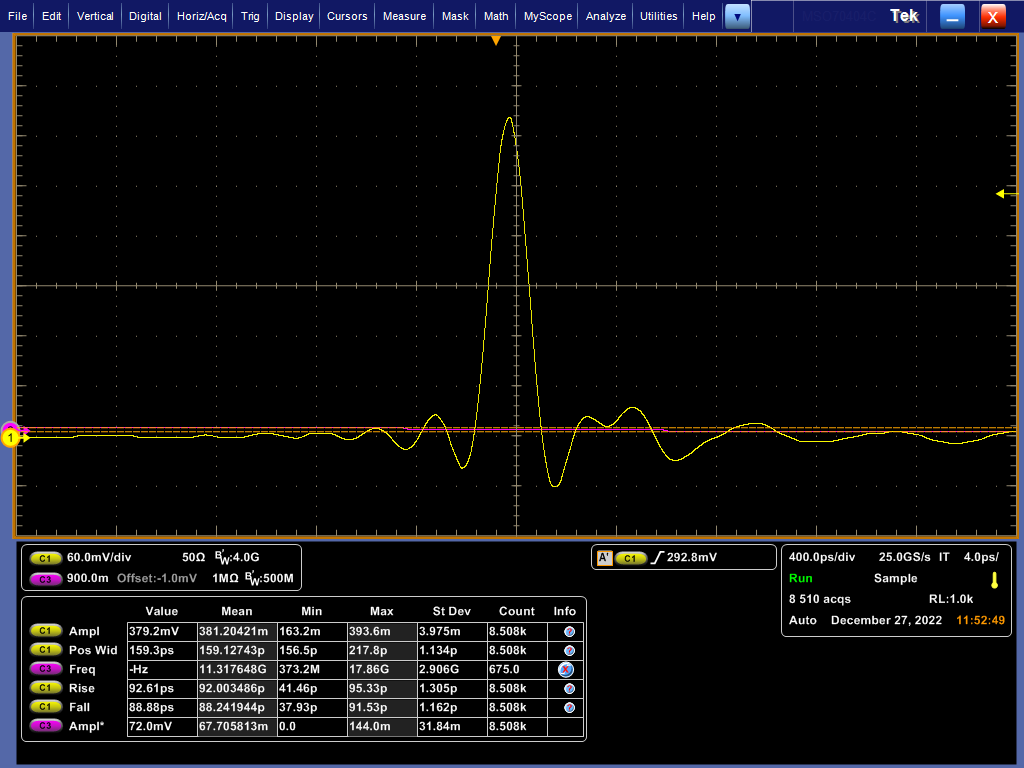
\includegraphics[width=\textwidth]{images/mediciones/vcc_5v_duty_50.png}
        \caption{Pulso medido, $V_{cc}$ \qty{5}{\volt}, D \qty{50}{\percent} }
        \label{fig:mediciones_5v_50}
    \end{subfigure}
    \hfill
    \begin{subfigure}[b]{0.49\textwidth}
        \centering
        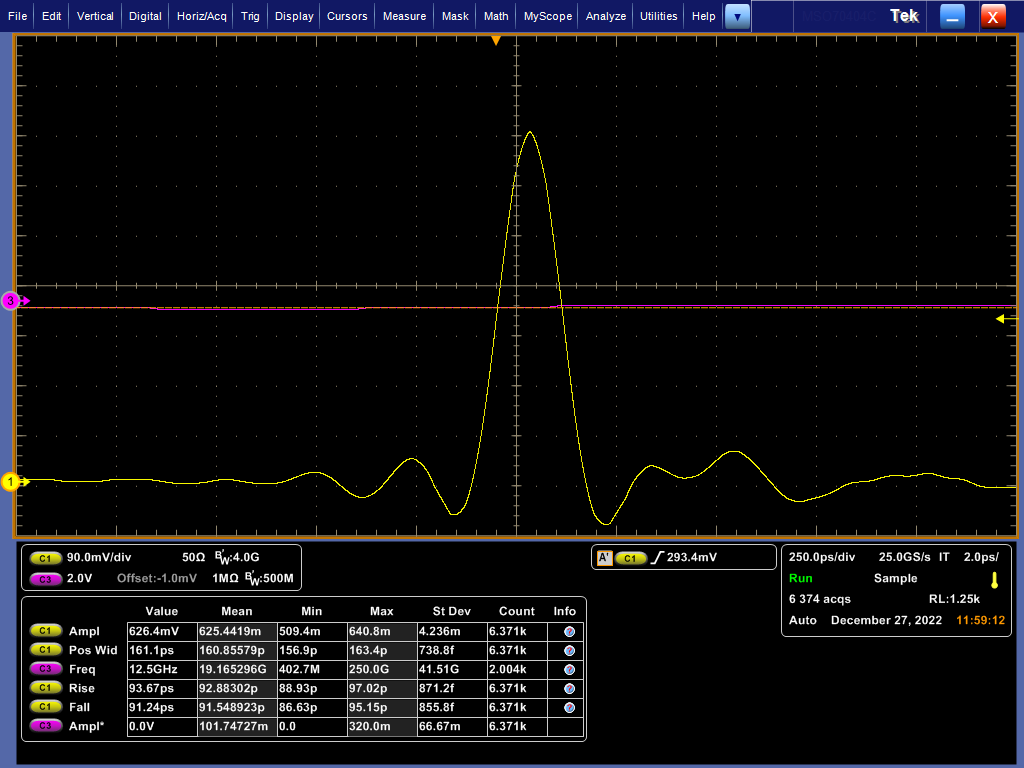
\includegraphics[width=\textwidth]{images/mediciones/vcc_5v_duty_70.png}
        \caption{Pulso medido, $V_{cc}$ \qty{5}{\volt}, D \qty{70}{\percent} }
        \label{fig:mediciones_5v_70}
    \end{subfigure}
    \caption{Pulsos medidos para $V_{cc} = \qty{5}{\volt}$}
    \label{fig:mediciones_5v}
\end{figure}

\begin{figure}[t!]
    \centering
    \begin{subfigure}[b]{0.49\textwidth}
        \centering
        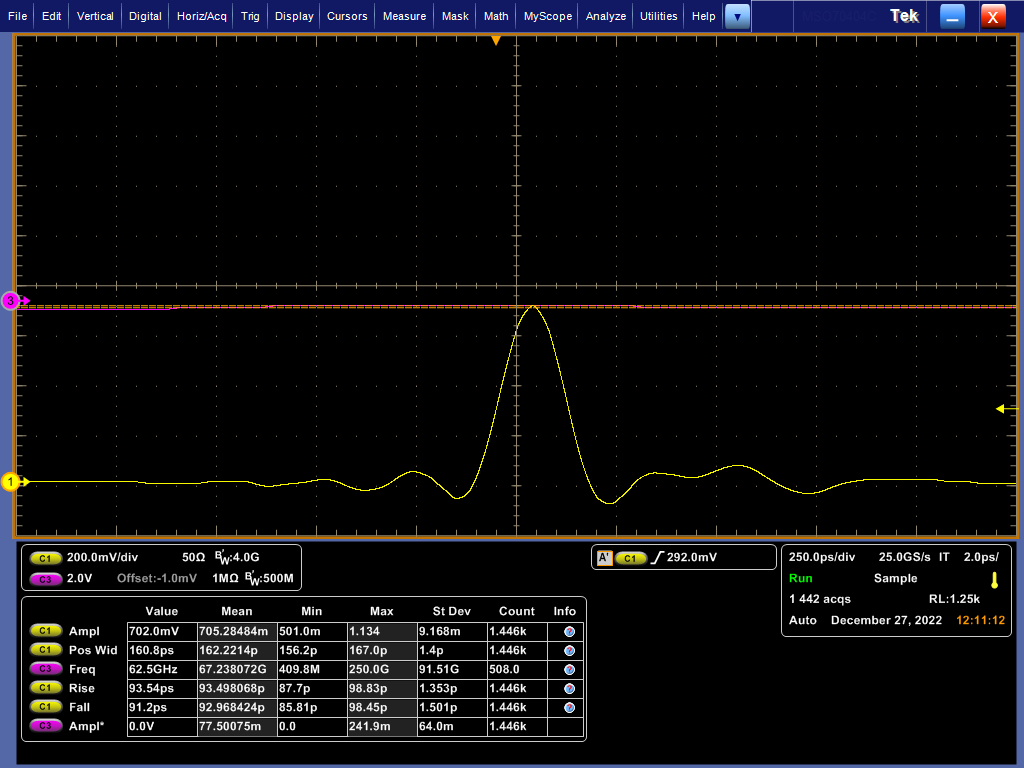
\includegraphics[width=\textwidth]{images/mediciones/vcc_7v_duty_50.png}
        \caption{Pulso medido, $V_{cc}$ \qty{7}{\volt}, D \qty{50}{\percent} }
        \label{fig:mediciones_7v_50}
    \end{subfigure}
    \hfill
    \begin{subfigure}[b]{0.49\textwidth}
        \centering
        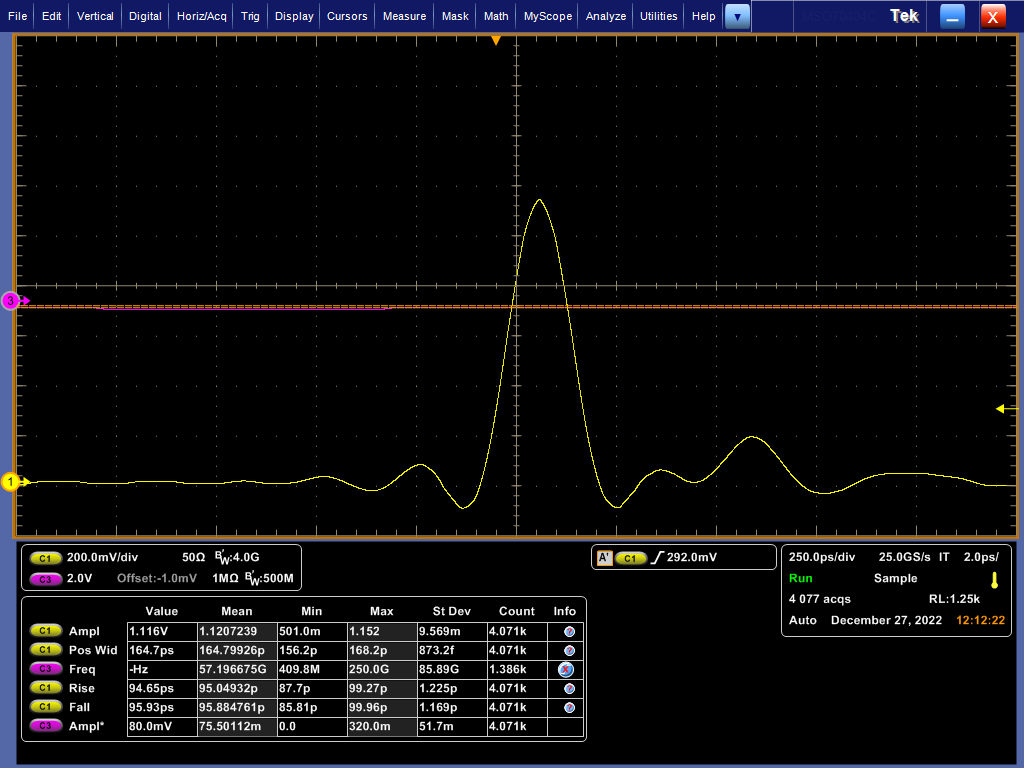
\includegraphics[width=\textwidth]{images/mediciones/vcc_7v_duty_70.png}
        \caption{Pulso medido, $V_{cc}$ \qty{7}{\volt}, D \qty{70}{\percent} }
        \label{fig:mediciones_7v_70}
    \end{subfigure}
    \caption{Pulsos medidos para $V_{cc} = \qty{7}{\volt}$}
    \label{fig:mediciones_7v}
\end{figure}

\begin{table}[t!]
\centering
\begin{tabular}{cccccccc}
\hline
    $V_{cc}$ [\unit{\volt}] & $D$ [\unit{\percent}] & $A$ [\unit{\volt}] & FWHM
    [\unit{\pico\second}] & $\qty{3}{\dB} \ B$ [\unit{\giga\hertz}] &
    $\qty{10}{\dB} \ B$ [\unit{\giga\hertz}] & $t_r$ [\unit{\pico\second}] &
    $t_f$ [\unit{\pico\second}]\\
\hline
    5 & 50 & 0.380 & 159 & 5.5 & 8.6 & 93 & 88 \\
    5 & 70 & 0.625 & 161 & 2.8 & 4.5 & 93 & 91 \\
    7 & 50 & 0.702 & 162 & 2.9 & 4.5 & 93 & 93 \\
    7 & 70 & 1.120 & 165 & 2.5 & 4.1 & 95 & 96 \\
\hline
\end{tabular}
\caption{Resultados de mediciones de pulso.}
\label{tab:mediciones_pulso_resultados}
\end{table}

\subsubsection{Comparación contra simulación}
\label{sec:comp_simulacion}

En las figuras \ref{fig:pulses_5v_50} a \ref{fig:psd_7v_70} pueden observarse
los resultados de las mediciones obtenidas superpuestos con los resultados de
simulación para las mismas condiciones de trabajo (amplitud de alimentación y
ciclo de trabajo).

Para las simulaciones, se toman dos resultados:

\begin{itemize}
    \item Una simulación ``ideal'', indicada como ``esquemático ideal'' en las
      leyendas, que se corresponde a una simulación sin contemplar parásitos de
      ningún tipo.
    \item Una simulación ``real'', en las leyendas ``Layout'', una simulación en
      la que se extrajeron previamente los efectos parásitos del \textit{PCB}
      mediante una simulación electromagnética y se incorporaron en la
      simulación del pulso.
\end{itemize}

Se realizan las comparaciones en el dominio del tiempo y de la frecuencia. Las
comparaciones en el dominio del tiempo consisten en la superposición del pulso
medido con los simulados. Para las comparaciones en el dominio de la frecuencia,
se calculó el espectro de cada una de las formas de onda del dominio del tiempo.
Para realizar las comparaciones, se exportaron los resultados a formato CSV y se
importaron dentro de un programa en python. Mediante las librerías numpy y
plotly se realizaron los distintos graficos.

En cuanto a la obtención de la PSD de cada pulso, en el código
\ref{get_spectrum_python} se muestra la función utilizada para obtenerla. La
misma reciba una secuencia de datos discretos \textit{x} y el tiempo de muestreo
entre cada muestra $sample\_time$. Obtiene la PSD aplicando una ventana de
\textit{Hanning} y normaliza por la norma $L^2$ de la
ventana \cite{oppenheim1999dsp}.

\begin{lstlisting}[language=Python, style=PythonStyle, caption=Función para obtener PSD,
label=get_spectrum_python, float]
import numpy as np

def get_spectrum(x, sample_time):
    w = np.hanning(len(x.shape))
    s_win = np.linalg.norm(w, 2) ** 2
    x_w = np.multiply(x, w)
    X_W = np.fft.rfft(x_w)
    P_xx = np.abs(X_W)**2 / s_win
    P_xx_dB = 10 * np.log10(P_xx)
    freq = np.fft.rfftfreq(x_w.shape[-1]) / sample_time
    return pd.DataFrame({'frequency': freq, 'magnitude': P_xx_dB})
\end{lstlisting}

En el dominio del tiempo, se observa una buena coincidencia entre la amplitud de
los pulsos y el ancho. Se observa una diferencia en el \textit{ringing} de
ambos.  Las simulaciones prácticamente no presentan oscilaciones alrededor del
pulso, mientras que las mediciones las presentan tanto previa como
posteriormente.  También se observa un segundo pulso de menor amplitud siguiendo
al primero.

Como causa de estas discrepancias, se descarta un efecto del \textit{PCB} no
modelado, ya que los parásitos de esta estructura fueron extraídos por una
simulación electromagnética, y sus efectos contemplados en las simulaciones del
\textit{layout}.

Estas  discrepancias sugieren una limitación en el modelado de alguno de los 
dispositivos, tanto el SRD como el Schottky. Las simulaciones predijeron correctamente
la amplitud y el ancho de los pulsos resultantes, pero fallaron en predecir 
el ringing y el pulso secundario.

\begin{figure}[t!]
    \centering
    \begin{subfigure}[b]{0.49\textwidth}
        \centering
        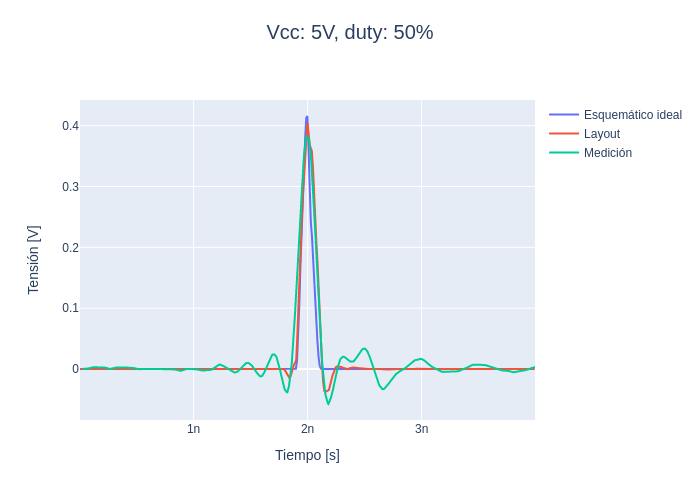
\includegraphics[width=\textwidth]{images/plots/Vcc_5V_duty_50_time_domain.png}
        \caption{Pulso @ $V_{cc}$ \qty{5}{\volt}, D \qty{50}{\percent} }
        \label{fig:pulses_5v_50}
    \end{subfigure}
    \hfill
    \begin{subfigure}[b]{0.49\textwidth}
        \centering
        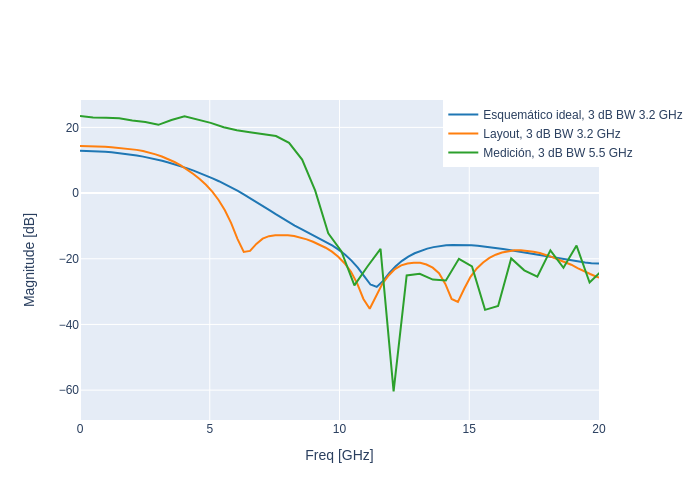
\includegraphics[width=\textwidth]{images/plots/Vcc_5V_duty_50_psd.png}
        \caption{PSD @ $V_{cc}$ \qty{5}{\volt}, D \qty{50}{\percent} }
        \label{fig:psd_5v_50}
    \end{subfigure}
    \caption{Pulsos y PSDs para $V_{cc}$ \qty{5}{\volt}, D \qty{50}{\percent} }
    \label{fig:plots_5v_50}
\end{figure}

\begin{figure}[t!]
    \centering
    \begin{subfigure}[b]{0.49\textwidth}
        \centering
        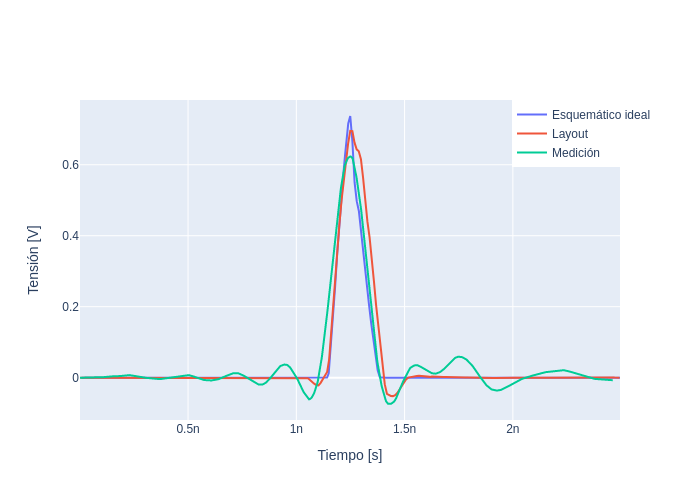
\includegraphics[width=\textwidth]{images/plots/Vcc_5V_duty_70_time_domain.png}
        \caption{Pulso @ $V_{cc}$ \qty{5}{\volt}, D \qty{70}{\percent} }
        \label{fig:pulses_5v_70}
    \end{subfigure}
    \hfill
    \begin{subfigure}[b]{0.49\textwidth}
        \centering
        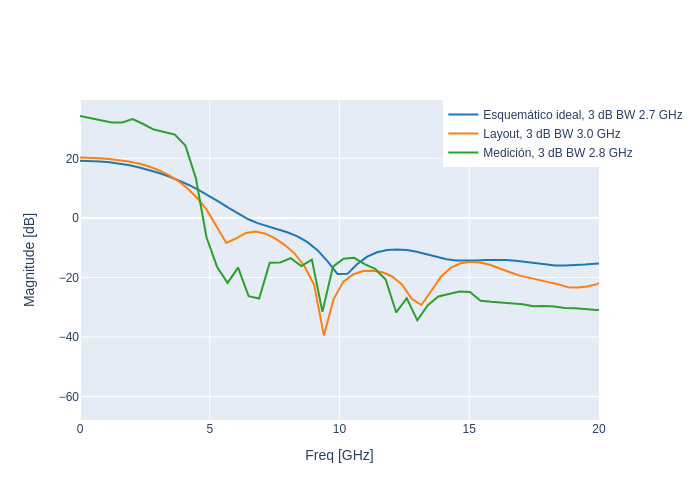
\includegraphics[width=\textwidth]{images/plots/Vcc_5V_duty_70_psd.png}
        \caption{PSD @ $V_{cc}$ \qty{5}{\volt}, D \qty{70}{\percent} }
        \label{fig:psd_5v_70}
    \end{subfigure}
    \caption{Pulsos y PSDs para $V_{cc}$ \qty{5}{\volt}, D \qty{70}{\percent} }
    \label{fig:plots_5v_70}
\end{figure}

\begin{figure}[t!]
    \centering
    \begin{subfigure}[b]{0.49\textwidth}
        \centering
        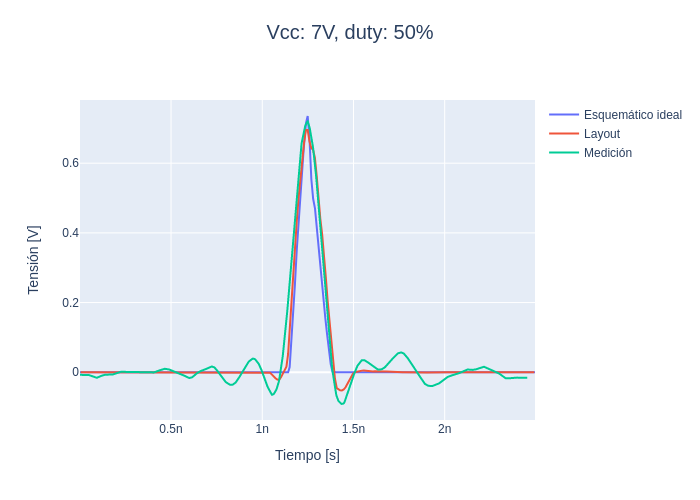
\includegraphics[width=\textwidth]{images/plots/Vcc_7V_duty_50_time_domain.png}
        \caption{Pulso @ $V_{cc}$ \qty{7}{\volt}, D \qty{50}{\percent} }
        \label{fig:pulses_7v_50}
    \end{subfigure}
    \hfill
    \begin{subfigure}[b]{0.49\textwidth}
        \centering
        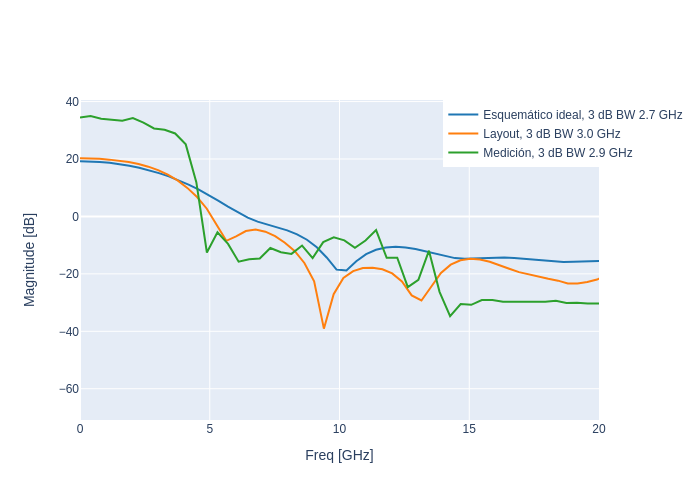
\includegraphics[width=\textwidth]{images/plots/Vcc_7V_duty_50_psd.png}
        \caption{PSD @ $V_{cc}$ \qty{7}{\volt}, D \qty{50}{\percent} }
        \label{fig:psd_7v_50}
    \end{subfigure}
    \caption{Pulsos y PSDs para $V_{cc}$ \qty{7}{\volt}, D \qty{50}{\percent} }
    \label{fig:plots_7v_50}
\end{figure}

\begin{figure}[t!]
    \centering
    \begin{subfigure}[b]{0.49\textwidth}
        \centering
        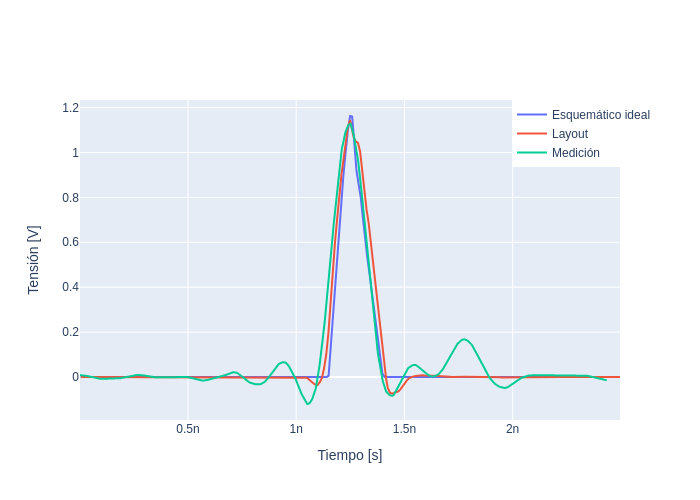
\includegraphics[width=\textwidth]{images/plots/Vcc_7V_duty_70_time_domain.png}
        \caption{Pulso @ $V_{cc}$ \qty{7}{\volt}, D \qty{70}{\percent} }
        \label{fig:pulses_7v_70}
    \end{subfigure}
    \hfill
    \begin{subfigure}[b]{0.49\textwidth}
        \centering
        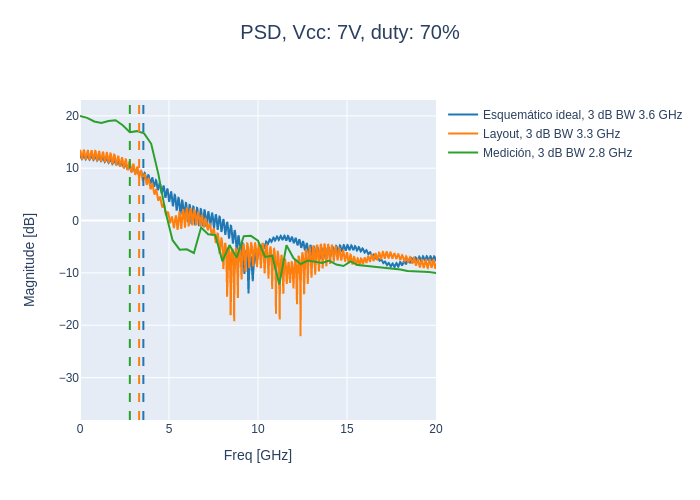
\includegraphics[width=\textwidth]{images/plots/Vcc_7V_duty_70_psd.png}
        \caption{PSD @ $V_{cc}$ \qty{7}{\volt}, D \qty{70}{\percent} }
        \label{fig:psd_7v_70}
    \end{subfigure}
    \caption{Pulsos y PSDs para $V_{cc}$ \qty{7}{\volt}, D \qty{70}{\percent} }
    \label{fig:plots_7v_70}
\end{figure}

\subsubsection{Comparación contra resultados de la literatura}

En la tabla \ref{tab:resultados_literatura} se resumen resultados reportados
para generadores de pulsos \textit{UWB} en la literatura. En la figura
\ref{fig:scatterplot_literature} se observan los valores de amplitud y duración
reportados en un gráfico de dispersión.

\begin{table}[t!]
    \begin{threeparttable}[b]
        {\footnotesize
            \begin{tabular}{ccccccccc}
                \hline
                Ref. & $A$ [\unit{\volt}] & $FWHM$ [\unit{\pico\second}] &
                Bal \tnote{a} & Bias & Dispositivos & $V_{cc}$ [\unit{\volt}] & $V_{in}$ [\unit{\volt}] & $PRF$ [\unit{\mega\hertz}] \\
                \hline
                \cite{rulikowski2004} & \num{\pm 0.896}, \num{\pm 1.6} \tnote{b} & 335, 511 & Sí & Int & SRD & 5 & TTL & 50 \\
                \cite{protiva2009} & \num{-7.5} & 110 & No & Ext & SRD+3TBJ+SD & 12 & TTL & 5 \\
                \cite{kamal2014} & \num{0.8} & 170 & No & Int & SRD & 4 & 4 & 10 \\
                \cite{han2002} & \num{0.2} & 300 & No & Ext & SRD+2SD & ? & ? & 10 \\
                \cite{han2005} & \num{-6}, \num{-4} & 150 & No & Int & SRD+L & >20 & 5 & 12 \\
                \cite{oloumi2018} & \num{1.27} \tnote{c} & 286 & No & Int & 2SRD+L & 10 & 10 \tnote{d} & ? \\
                \textbf{Prop.} & \num{1.12} & 165 & No & Int & SRD+SD & 7 & CMOS  &
                \num{10} \\
            \end{tabular}
        }
        \begin{tablenotes}
            \item [a] \textit{Balanceado}.
            \item [b] la publicación presenta dos resultados, correspondientes a
            circuitos con componentes concentrados y distribuidos.
            \item [c] la publicación presenta múltiples resultados, se muestran
            los mejores.
            \item [d] la señal de entrada es senoidal.
        \end{tablenotes}
    \end{threeparttable}
    \caption{Resultados reportados en la literatura}
    \label{tab:resultados_literatura}
\end{table}

\begin{figure}
\centering
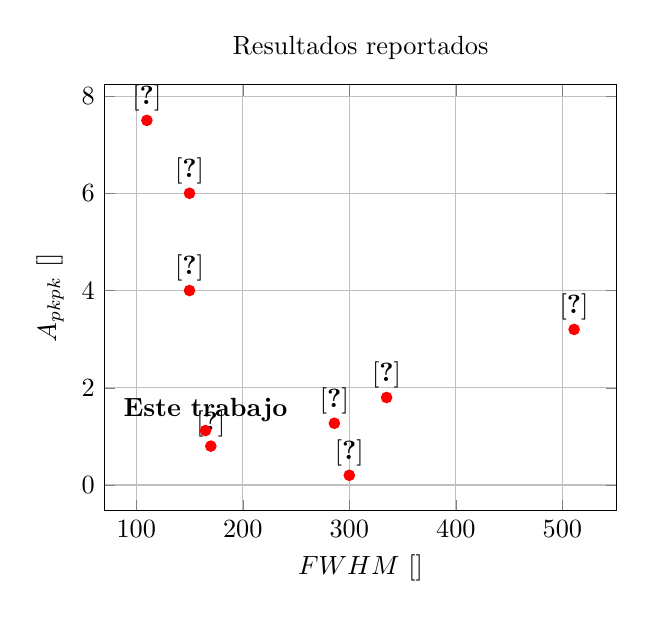
\begin{tikzpicture}[scale=0.95]
  \begin{axis}[
    xlabel={$FWHM$ [\unit{\pico\second}]},
    ylabel={$A_{pkpk}$ [\unit{\volt}]},
    title=Resultados reportados,
    grid=both
    ]
    \addplot[
        scatter/classes={a={blue}, b={red}},
        scatter, mark=*, only marks, 
        scatter src=explicit symbolic,
        nodes near coords*={\Label},
        visualization depends on={value \thisrow{label} \as \Label} %<- added value
    ] table [meta=class] {
        x   y       class   label
        511 3.2     b       {\cite{rulikowski2004}}
        335 1.8     b       {\cite{rulikowski2004}}
        110 7.5     b       {\cite{protiva2009}}
        170 0.8     b       {\cite{kamal2014}}
        300 0.2     b       {\cite{han2002}}
        150 6       b       {\cite{han2005}}
        150 4       b       {\cite{han2005}}
        286 1.27    b       {\cite{oloumi2018}}
        165 1.12    b       {\textbf{Este trabajo}}
    };

  \end{axis}
\end{tikzpicture}
  \caption{Diagrama de dispersión de resultados reportados.}
  \label{fig:scatterplot_literature}
\end{figure}

En cuanto a los resultados reportados en este trabajo, se obtuvo uno de los
anchos de pulso más bajos, existiendo otros trabajos que reportan el mismo o
menor ancho de pulso con mayor amplitud, pero también mayor complejidad. Otra
característica a destacar es la simplicidad del diseño implementado, tanto en
cantidad de componentes activos, como en requisitos de fuente de alimentación y
pulso de entrada.

En \cite{rulikowski2004} se presenta un diseño compuesto de un solo SRD en el
que se desarrolla un pulso balanceado a la salida. Se presentan dos diseños, uno
con componentes distribuidos y otro con componentes concentrados. En ambos casos
se obtienen amplitudes pico a pico de pulso mayores a las de este trabajo. Es
destacable que se obtienen mayores amplitudes usando una fuente de alimentación
menor, de \qty{5}{\volt}. En cuanto al ancho de pulso, ambos pulsos presentan
duraciones mayores que las de nuestro trabajo. En cuanto a la complejidad, el
\textit{pulser} está implementado solamente con 1 SRD y componentes
distribuidos o concentrados, dependiendo de la versión, por lo que es más simple
que nuestro trabajo. El \textit{driver} presenta la misma complejidad en ambos
casos, ya que está implementado con un solo circuito integrado. Nuestro trabajo
presenta más versatilidad, ya que la amplitud de la fuente de alimentación puede
variarse entre \qty{0}{\volt} y \qty{30}{\volt}, mientras que el integrado
utilizado en el driver de \cite{rulikowski2004} trabaja con \qty{5}{\volt}
fijos.

En \cite{protiva2009} se reporta un resultado de gran amplitud y duración de
pulso menor a la de este trabajo. La complejidad del diseño implementado es
mucho mayor: necesita una alimentación de \qty{12}{\volt} y
una corriente de \textit{bias} externa, y la etapa \textit{driver} está
implementada con 3 TBJs, frente a 1 solo \textit{gate driver} en nuestro
trabajo.

En \cite{kamal2014} el pulso reportado es de características muy similares a las
de nuestro trabajo.  La duración del pulso es prácticamente la misma, mientras
que en amplitud nuestro trabajo logró una mayor en un \qty{40}{\percent}.
Nuestro trabajó logró para el \textit{pulser} una complejidad menor a la
reportada en \cite{kamal2014}, ya que en nuestro caso omitimos la red RC y el
atenuador. En cuanto a etapa \textit{driver}, \cite{kamal2014} no presenta
ninguna, en los resultados se reporta haber utilizado como entrada al
\textit{pulser} un pulso bipolar.

En \cite{han2002} el generador presentado desarrolla pulsos monociclo, que son
la primera derivada de un pulso gaussiano. Nuestro trabajó logro una amplitud de
pulso mayor y también una duración de pulso menor. No se especifica el valor de
amplitud de señal de entrada utilizado. La entrada al circuito es bipolar, y no
se incluye un \textit{driver} de adaptación de pulso. La complejidad del
generador descripto es mayor que la de este trabajo, utilizando bias externo, un
diodo SRD, dos Schottky y una red RC. Sin embargo, el generador de
\cite{han2002} implementa un monociclo que es una derivada de un pulso gaussiano
como el desarrollado en nuestro trabajo, por lo que es natural que la
complejidad sea mayor.

El resultado reportado en \cite{han2005} consiste en pulsos de mayor amplitud y
menor duración a los de nuestro trabajo. En ambos casos, el pulser se encuentra
acoplado por \textit{AC}, lo que vuelve más complejo el diseño.  Se presentan
dos generadores, uno con línea de transmisión, y otro con un inductor, que
utiliza al SRD en paralelo. El diseño con inductor es más complejo, ya que este
se encuentra en el camino del pulso por lo que debe ser seleccionado con
cuidado. En ambos casos se utiliza una red RC paralelo, mientras que en nuestro
trabajo no. En cuanto a la amplitud de entrada, esta es TTL \qty{5}{\volt}. Sin
embargo, se reporta una etapa driver entre la entrada y el pulser, compuesta por
un amplificador opearcional en configuración no inversor, y dos buffers de
corriente. En \cite{NguyenHan2014} se explica el circuito en más detalle y se
reporta una amplitud pico a pico a la entrada del pulser de \qty{20}{\volt}.
Entonces, este trabajo logra mayores amplitudes pero con una etapa driver mucho
más compleja.

El resultado de \cite{oloumi2018} consiste en un pulso de mayor amplitud y mayor
ancho al de nuestro trabajo. La complejidad del diseño es mayor, ya que utiliza
dos SRD y un inductor que se encuentra en el camino de alta frecuencia, por lo
que es costoso de seleccionar. La señal de entrada es una senoidal, que para el
contexto en el que desarrollamos nuestro generador, es más costosa de conseguir,
ya que requiere algún DAC, frente a la excitación de nuestro generador que es
una señal cuadrada, fácilmente obtenible como salida digital de una FPGA o
microcontrolador.

\section{Aplicaciones}

Como fuese explicado en el capitulo 1, el generador de pulsos desarrollado tiene
aplicaciones en caminos de transmisión y recepción de sistemas UWB. En cuanto a
los caminos de transmisión, en el
capitulo se desarrolló cómo la utilización de un generador de pulsos ultracortos
cadenas permite su simplificación con respecto a las implementadas en
base a generadores de pulsos en banda base y su conversión a banda pasante
mediante un multiplicador \cite{Altieri2021}. La utilización del generador
evita la necesidad de un oscilador local, un multiplicador y una etapa de
amplificación, dado que los multiplicadores para los anchos de banda UWB suelen
ser pasivos con pérdidas significativas. En los caminos de recepción, el
generador de pulsos permite la implementación de una arquitectura de muestreo en
tiempo equivalente, reemplazando así a un conversor de Nyquist que es sumamente
costoso para los anchos de banda en cuestión. En esta sección se demostrará la
aplicación del generador diseñado en un camino de transmisión.

\subsection{Aplicaciones en transmisión}

Para validar la aplicabilidad del transmisor en un cadena de transmisión, se
simulará el circuito de la figura \ref{fig:proposed_uwb_tx_path}. En este
sistema, para generar un pulso en banda pasante, se excita un filtro pasabandas
con la respuesta en frecuencia deseada con el generador de pulsos ultracortos,
que aproxima un tren de impulsos ideal.  En esta forma de onda ideal, los
impulsos tienen un ancho temporal de 0 y una amplitud infinita, y en el dominio
de la frecuencia, son perfectamente planos.  Esta es una aproximación, el
geneardor real tendrá un ancho de banda finito y una duración temporal finita al
igual que la amplitud. La aproximación de impulso ideal puede ser considerada
válida si el pulso tiene un espectro plano dentro de la banda de frecuencias del
filtro pasabanda. Fuera de esta banda, dada la atenuación del filtro, es
indistinta la densidad espectral del pulso de entrada.

El filtro pasabanda utilizado tendrá las mismas características que el reportado
en \cite{Altieri2021}: Chebyshev de orden 5, con \qty{0.1}{\dB} de
\textit{ripple}, frecuencia central de \qty{1.9}{\giga\hertz} y
\qty{1}{\giga\hertz} de ancho de banda. Esto resulta en una banda de paso de
entre \qty{1.4}{\giga\hertz} y \qty{2.4}{\giga\hertz}. En la figura
\ref{fig:passband_chebyshev_schematic} puede observarse la vista esquemático del
filtro. Como fuese explicado en la sección \ref{sec:pulse_bandwidth}, el pulso
teórico tiene un ancho de banda a \qty{3}{\dB} de \qty{3.46}{\giga\hertz} y a
\qty{10}{\dB} de \qty{6.32}{\giga\hertz}. En cuanto al ancho de banda obtenido
en las mediciones, para el pulso generado con $V_{cc}$ de \qty{5}{\volt} y un
ciclo de trabajo de \qty{70}{\percent}, se obtuvo un ancho de \qty{3}{\dB} de
\qty{2.8}{\giga\hertz} y a \qty{10}{\dB} de \qty{4.5}{\giga\hertz}. Tanto para
las mediciones como para el valor teórico, el ancho de banda del pulso se
encuentra por arriba de la banda de paso del filtro, por lo que es esperado que
el generador diseñado aproxime correctamente al impulso ideal frente al filtro
pasabanda.

\begin{figure}[t]
    \centering
    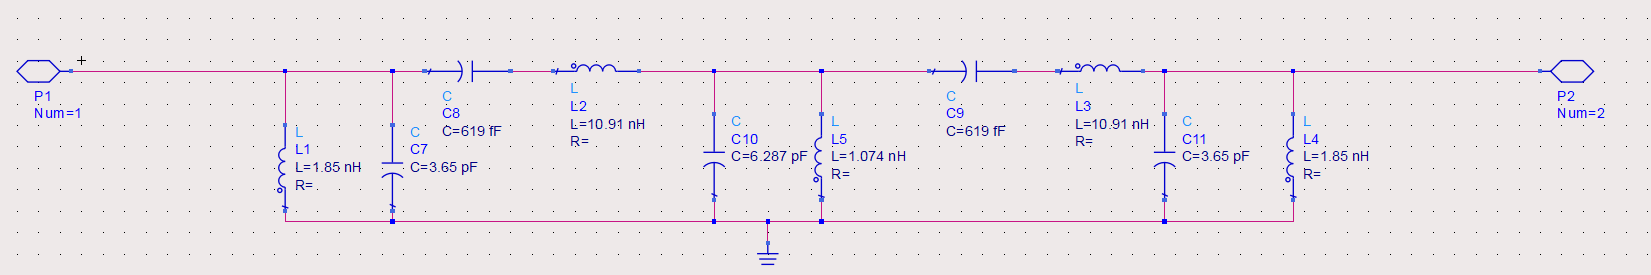
\includegraphics[width=\linewidth]{images/passband_chebyshev_schematic.png}
    \caption{Filtro Chebyshev utilizado para simulación de cadena de
    transmisión.}
    \label{fig:passband_chebyshev_schematic}
\end{figure}

\begin{figure}[t]
    \centering
    \begin{subfigure}[b]{0.45\textwidth}
        \centering
        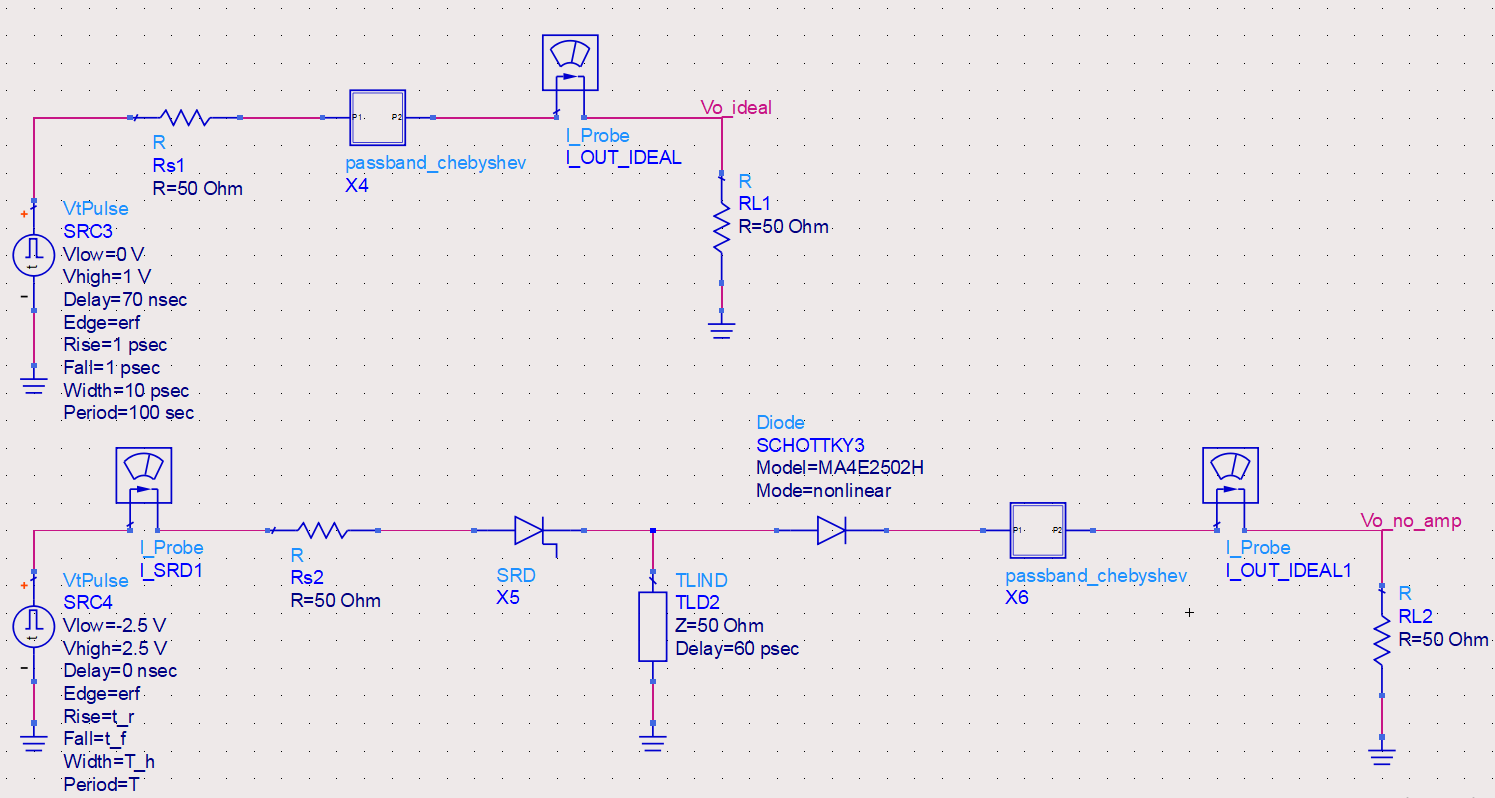
\includegraphics[width=\textwidth]{images/passband_pulser_sim_no_amp.png}
        \caption{Simulación de filtro pasabanda con impulso ideal y pulser sin
        buffer.}
        \label{fig:passband_pulser_sim_no_amp}
    \end{subfigure}
    \hfill
    \begin{subfigure}[b]{0.45\textwidth}
        \centering
        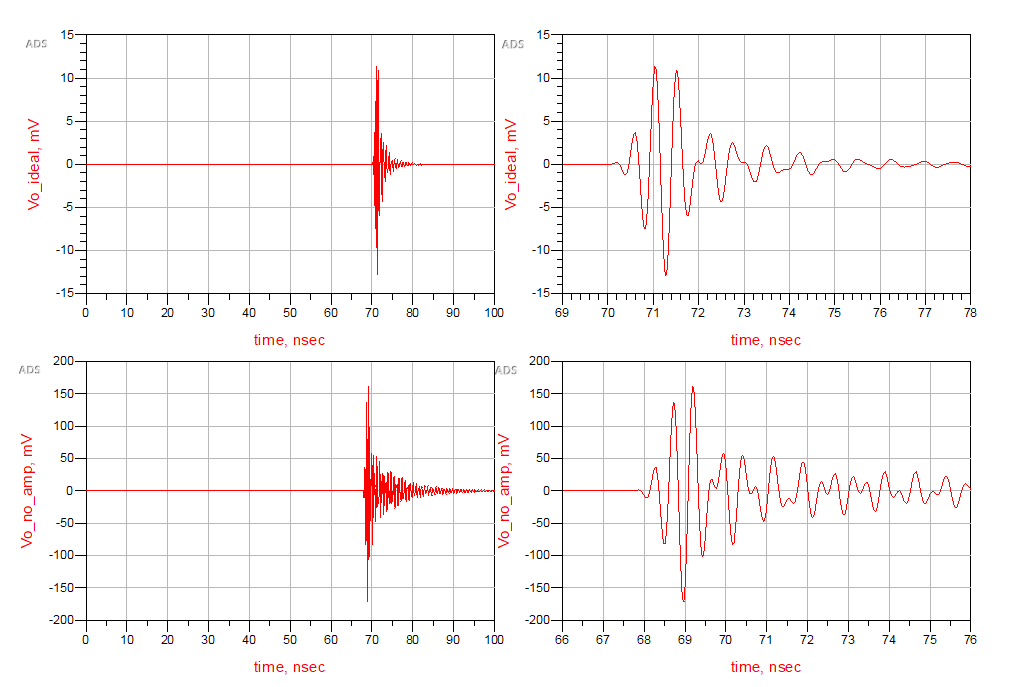
\includegraphics[width=\textwidth]{images/passband_pulser_sim_no_amp_results.png}
        \caption{Resultado obtenido en simulación de pulser cargado con filtro
        pasabanda.}
        \label{fig:passband_pulser_sim_no_amp_results}
    \end{subfigure}
    \caption{Esquemático utilizado para filtro pasabanda y simulación realizada
    con impulso ideal y generado por pulser.}
    \label{fig:passband_cheby_and_with_pulser}
\end{figure}

\subsection{Simulación}

Como primera simulación, se realizó una compuesta por dos circuitos: uno ideal,
en el que se aplica al filtro pasabanda un pulso ideal de \qty{1}{\volt} de
amplitud y \qty{1}{\pico\second} de duración, y otro en el que se conecta el
filtro directamente a la salida del pulser. Simulamos ambos casos para poder
comparar el desempeño del generador desarrollado contra el caso ideal. Cabe
destacar que el caso ideal con respecto al del pulser lo es tanto por las
características del pulso cómo por el efecto de carga. Es decir, al estar el
geneardor ideal implementado con una fuente de tensión ideal, no presenta
efectos de carga, mientras que el pulser se ve afectado por estar cargado con
una impedancia reactiva.

En la figura \ref{fig:passband_pulser_sim_no_amp} puede observarse el
esquemático simulado y en la \ref{fig:passband_pulser_sim_no_amp_results} los
resultados obtenidos. Se observa que el pulso resultante del pasabanda con el
pulser tiene mayores oscilaciones que en el caso del impulso ideal. En el caso
ideal, el pulso tiene una duración aproximada de \qty{10}{\nano\second},
mientras que en el caso del pulser, la duración es mayor a
\qty{20}{\nano\second}, con oscilaciones que continúan incluso luego de este
tiempo. En cuanto a la forma del pulso, se ve que el pulso principal tiene la
misma forma. La amplitud de los pulsos es distinta, pero esta no es una cantidad
que sea comparable, ya que los pulsos de entrada tienen amplitudes distintas.
Entonces, en este caso observamos que cargando al pulser directamente con el
filtro pasbandas se logra reproducir la misma forma de onda que con un impulso
ideal, pero luego del pulso principal se observan unas oscilaciones remanentes
que en el caso del impulso ideal no están presentes.

Para solucionar el problema de las oscilaciones se propone introducir un bloque
de ganancia entre el pulser y el filtro pasabanda. Además de incrementar la
amplitud  resultante, esta etapa remueve los efectos de carga sobre el pulser,
que en este caso son los responsables de las oscilaciones. Para el amplificador
se utiliza un TRF37B75 de Texas Instruments. Este se caracteriza por una
ganancia de \qty{15}{\dB} en un rango de \qty{40}{\mega\hertz} a
\qty{4000}{\mega\hertz} y muy bajo costo. En cuanto a su costo de
implementación, se alimenta con \qty{5}{\volt} por lo que no requiere de fuentes
adicionales, y como componentes adicionales únicamente requiere de dos
capacitores para acoplar la entrada y la salida, y un \textit{choke} para la
entrada de alimentación. Económicamente su costo también es extremadamente bajo,
menor a 1 dolar al momento de la redacción de este trabajo. Por lo tanto, la
inclusión de este componente en la cadena de transmisión propuesta sigue
manteniendo la premisa de bajo costo y simplicidad de implementación. Cabe
resaltar que trabajar con este amplificador resulta en un filtrado de las
componentes menores a \qty{40}{\mega\hertz}, rango de frecuencia en el que la
salida del pulser tiene energía. Sin embargo, como en esta aplicación se
excitará un filtro pasabandas con una banda de paso por encima de estas
frecuencias, esto no es un problema, ya que este componente filtra todas las
frecuencias por debajo de \qty{1.4}{\giga\hertz}, lo que vuelve indistinto el
contenido espectral de las frecuencias por debajo de este valor.

Para simular el efecto del amplificador se utiliza un modelo de SPICE provisto
por el fabricante. En la figura \ref{fig:passband_pulser_sim_with_amp} se
observa el esquemático simulado. En el mismo se observa el pulser con su salida
conectada al TRF37B75, acoplada a alterna mediante un capacitor serie. La salida
del amplificador también se encuentra acoplada en alterna, y está conectada al
filtro pasabanda cargado con una impedancia de \qty{50}{\ohm}. En la figura
\ref{fig:passband_pulser_sim_with_amp_result} se observa el resultado de la
simulación. El efecto de oscilaciones se ve totalmente removido, con una
duración total de pulso de \qty{10}{\nano\second}, al igual que en el caso
ideal. La forma del pulso también se observa sin cambios. Vemos entonces que
agregando un amplificador como etapa buffer entre el pulser y el filtro
pasabanda, se logra el mismo resultado que con un impulso ideal. En cuanto a la
amplitud del pulso, por la acción del amplificador vemos que esta resulta en
casi \qty{600}{\milli\volt}, mientras que en el resultado de
\ref{fig:passband_pulser_sim_no_amp_results} era de \qty{150}{\milli\volt}. Cabe
destacar que por la configuración del amplificador, su salida es negativa, por
lo que se observa que el pulso de la figura
\ref{fig:passband_pulser_sim_with_amp_result} se encuentra invertido con
respecto al caso ideal de la figura
\ref{fig:passband_pulser_sim_no_amp_results}. Esto no es un problema, ya que
únicamente representa un cambio de fase con respecto a la señal original, se
sigue manteniendo la magnitud de la respuesta en frecuencia que es la cantidad
de interés en esta aplicación.

De esta manera, queda demostrada en esta sección la validez de la cadena de transmisión
propuesta en el capitulo 1 y su implementación con el generador desarrollado. Se
demostró que acoplar directamente el filtro pasabandas al pulser resulta en
oscilaciones indeseadas, pero este problema puede ser solucionado con la
inclusión de un amplificador de bajo costo. Esto tiene además el beneficio de
aumentar la amplitud del pulso final.

\begin{figure}[t]
    \centering
    \begin{subfigure}[b]{0.45\textwidth}
        \centering
        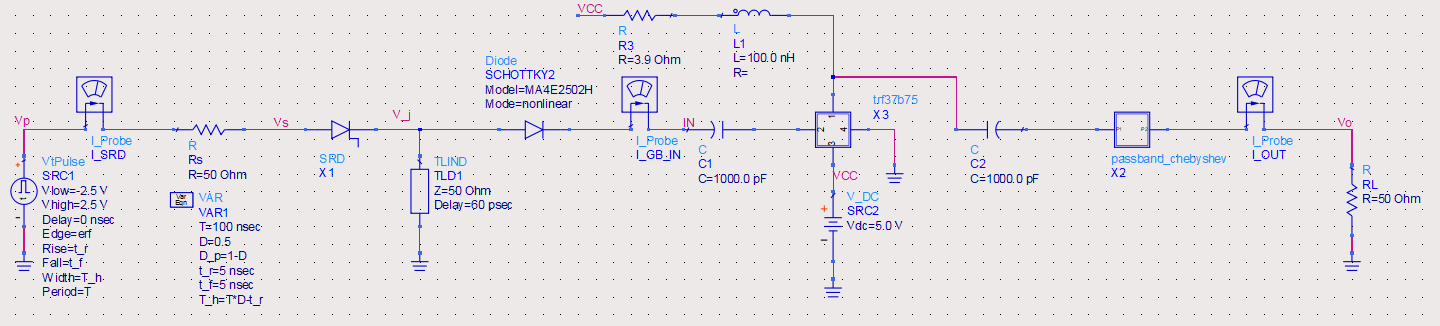
\includegraphics[width=\linewidth]{images/passband_pulser_sim_with_amp.png}
        \caption{Simulación de filtro pasabanda con pulser y amplificador.}
        \label{fig:passband_pulser_sim_with_amp}
    \end{subfigure}
    \hfill
    \begin{subfigure}[b]{0.45\textwidth}
        \centering
        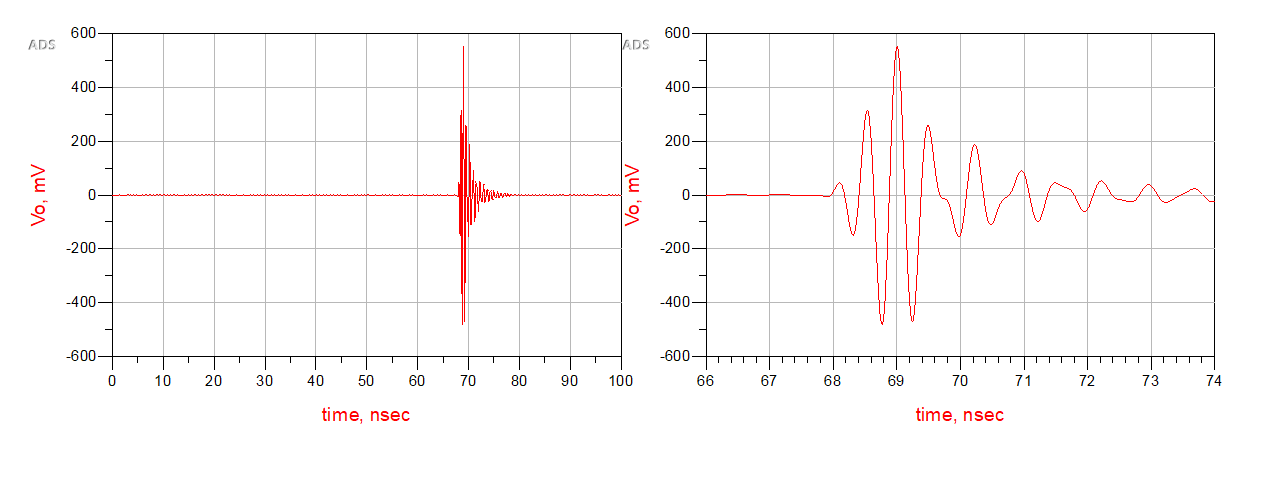
\includegraphics[width=\linewidth]{images/passband_pulser_sim_with_amp_result.png}
        \caption{Resultado de simulación de filtro pasbanda con pulser y
        amplificador.}
        \label{fig:passband_pulser_sim_with_amp_result}
    \end{subfigure}
    \caption{Simulación de pulser cargado con filtro pasabanda y etapa buffer.}
    \label{fig:passband_pulser_with_amp}
\end{figure}

\subsection{Validación con pulso medido}

Para realizar la validación del sistema propuesto, se realiza una simulación
utilizando como fuente al pulso medido en lugar de la vista esquemático del
generador desarrollado. Para esto, se utilizó el software LTspice, que permite
definir una fuente de tensión ideal utilizando un archivo CSV, siendo dicho
archivo el generado por el osciloscopio en la medición del pulso. Fue necesario
recurrir a este software en lugar del que fue utilizado en el resto del trabajo,
ADS, dado que este únicamente permite para fuentes de este estilo utilizar como
entrada un tipo de archivo propietario \textit{Keysight Dataset} que es generado
por los instrumentos de dicha compañía. Dada la imposibilidad de traducir el
archivo CSV, se utilizó LTspice.

En cuanto al pulso medido, se utilizó el correspondiente a $V_{cc}$ de
\qty{5}{\volt} y un ciclo de trabajo de \qty{70}{\percent}, dado que presentaba
el mejor compromiso entre ancho de banda y amplitud. En la figura
\ref{fig:passband_with_measurement} se observa el esquemático simulado, y en
\ref{fig:passband_with_measurement_result} el resultado. La simulación consiste
de una fuente ideal con la forma de onda del pulso medido, y la carga es el
filtro Chebyshev de orden 5 cargado con una resistencia de \qty{50}{\ohm}. Como
en este caso se utiliza una fuente ideal para la generación del pulso, no es
necesaria la inclusión de una etapa de amplificación, ya que no hay efectos de
carga. En cuanto a la ganancia que impondría esta etapa, puede contemplarse
afectando linealmente el pulso obtenido. En cuanto al resultado, se observa la
misma forma de onda que para la simulación de pulso ideal de la figura
\ref{fig:passband_pulser_sim_no_amp}, y la misma duración de
\qty{10}{\nano\second}. De esta manera, queda validada la utilidad del pulso
medido en la aplicación de generación de pulsos en banda pasante de manera
directa.

\begin{figure}[t]
    \centering
    \begin{subfigure}[b]{0.45\textwidth}
        \centering
        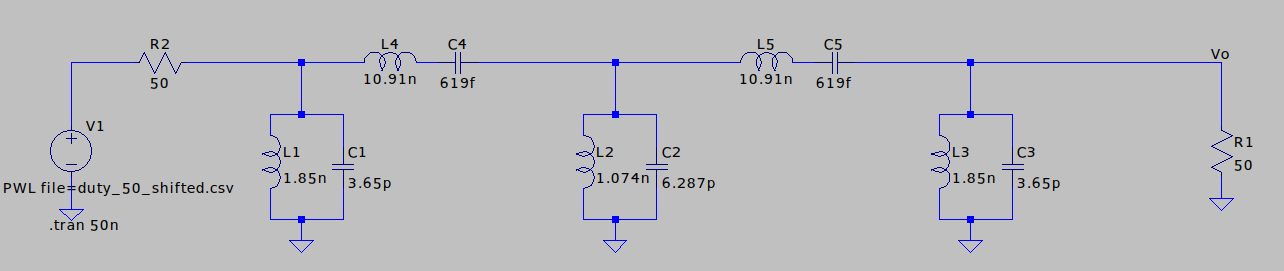
\includegraphics[width=\linewidth]{images/passband_with_measurement.png}
        \caption{Simulación de filtro pasabanda excitado con pulso medido.}
        \label{fig:passband_with_measurement}
    \end{subfigure}
    \hfill
    \begin{subfigure}[b]{0.45\textwidth}
        \centering
        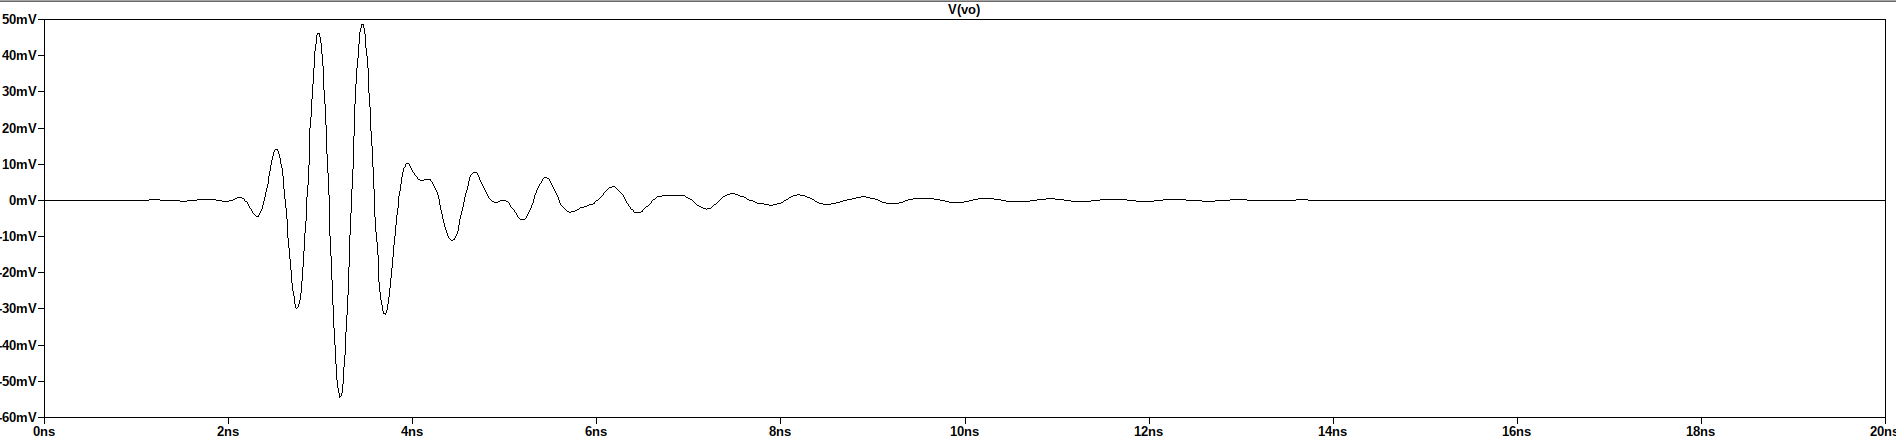
\includegraphics[width=\linewidth]{images/passband_with_measurement_result.png}
        \caption{Resultado de simulación de filtro pasabanda excitado con pulso
        medido.}
        \label{fig:passband_with_measurement_result}
    \end{subfigure}
    \caption{Simulación de filtro pasabanda excitado por medición de pulso.}
    \label{fig:passband_measurement}
\end{figure}
